\documentclass[12pt,a4paper]{scrartcl}
\usepackage{amsmath}
\usepackage{amsfonts}
\usepackage{amsthm}
\usepackage{amssymb}
\usepackage[latin1]{inputenc}
\usepackage{mathptmx}
\usepackage{amscd}
\usepackage{array}
\usepackage{color}
\usepackage{hyperref}
\usepackage{url}
\usepackage{graphicx}
\usepackage{multicol}

\usepackage{booktabs}

\usepackage{pgf, tikz}
\usepackage{color}

% !TeX spellcheck = en_US

%\textwidth=15cm \textheight=22cm \topmargin=0.5cm
%\oddsidemargin=0.5cm \evensidemargin=0.5cm

\usepackage[T1]{fontenc}

\usepackage[scaled=0.8]{beramono}

\usepackage{fancyvrb} \RecustomVerbatimEnvironment{Verbatim}{Verbatim}
{xleftmargin=15pt, frame=single, fontsize=\small}


\newcounter{listi}
\newcommand{\stdli}{ \topsep0ex \partopsep0ex % .5ex plus.25ex minus.125ex%
\parsep.2ex plus.1ex minus.1ex \itemsep0ex% .5ex plus.25ex minus.125ex%
\leftmargin2.5em \labelwidth2em \labelsep.5em \rightmargin0em}% \samepage }
\newenvironment{arab}{\begin{list}{\textup{(\arabic{listi})}}%
	{\usecounter{listi}\stdli}}{\end{list}}
\newenvironment{rome}{\begin{list}{\textup{(\roman{listi})}}%
	{\usecounter{listi}\stdli}}{\end{list}}
\newenvironment{latin}{\begin{list}{\textup{(\alph{listi})}}%
	{\usecounter{listi}\stdli}}{\end{list}}
\renewenvironment{itemize}{\begin{list}{{$\bullet$}}{\stdli}}{\end{list}}
\newenvironment{myverb}{\begin{small}}{\end{small}\pagebreak[2]}  %%%%%  \vspace{-0.8\baselineskip}


\newtheorem{theorem}{Theorem}
\newtheorem{lemma}[theorem]{Lemma}
\newtheorem{corollary}[theorem]{Corollary}
\newtheorem{proposition}[theorem]{Proposition}


\theoremstyle{definition}
\newtheorem{remark}[theorem]{Remark}
\newtheorem{definition}[theorem]{Definition}

\let\phi=\varphi

\def\CC{{\mathbb C}}
\def\ZZ{{\mathbb Z}}
\def\QQ{{\mathbb Q}}
\def\RR{{\mathbb R}}
\def\EE{{\mathbb E}}
\def\AA{{\mathbb A}}
\def\PP{{\mathbb P}}
\def\NN{{\mathbb N}}

\def\cL{{\mathcal L}}

\def\Ker{\operatorname{Ker}}
\def\Im{\operatorname{Im}}
\DeclareMathOperator{\gp}{gp}
\DeclareMathOperator{\rank}{rank}
\DeclareMathOperator{\conv}{conv}
\DeclareMathOperator{\aff}{aff}
\DeclareMathOperator{\cone}{cone}
\DeclareMathOperator{\rec}{rec}
\DeclareMathOperator{\mrank}{mrank}
\DeclareMathOperator{\Hilb}{Hilb}
\DeclareMathOperator{\vol}{vol}
\DeclareMathOperator{\Cl}{Cl}


\def\cG{{\mathcal G}}
\def\cR{{\mathcal R}}

\let\hat=\widehat
\let\tilde=\widetilde
\let\Bar=\overline

\let\iso=\cong

\let\epsilon=\varepsilon
\def\discuss#1{\marginparsep=1em\marginparwidth=60pt
\marginpar{\tt \footnotesize \raggedright #1}}

\definecolor{darkgray}{gray}{0.00}

\addtokomafont{section}{\color{darkgray}}

\setkomafont{sectionentry}{\large}

\addtokomafont{subsection}{\color{darkgray}}

\addtokomafont{subsubsection}{\normalsize}

\parindent=0pt \parskip=4pt

\setcounter{tocdepth}{3}

%\def\Normaliz#1+{\textsf{Normaliz}}
%\def\jNormaliz#1+{\textsf{jNormaliz}}
%\def\NmzIntegrate#1+{\textsf{NmzIntegrate}}

\def\itemtt[#1]{\item[\textbf{\ttt{#1}}]}

\def\ttt{\texttt}


\begin{document}
\vspace*{2cm}

\centerline{\Large\textbf{Normaliz 3.0}} \vspace*{1cm}


\begin{center}Winfried Bruns, Tim R�mer, Richard Sieg and Christof
	S�ger\\[14pt]
	Normaliz 2 team member: Bogdan Ichim\\[14pt]
	\url{http://www.math.uos.de/normaliz}\\[14pt]
	\url{mailto:normaliz@uos.de}
\end{center}



\tableofcontents

\newpage

%%%%%%%%%%%%%%%%%%%%%%%%%%%%%  INTRODUCTION  %%%%%%%%%%%%%%%%%%%%%%%%%%%%%
\section{Introduction}\label{facil}

\subsection{The objectives of Normaliz}

The program Normaliz  is a tool for computing
the Hilbert bases and enumerative data of rational cones and, more generally, sets of lattice points in rational polyhedra. The mathematical background and the terminology of this manual are explained in Appendix A. For a thorough treatment of the  mathematics involved we refer the reader to
\cite{BG} and \cite{BH}. The terminology follows \cite{BG}. For
algorithms of Normaliz see \cite{BHIKS}, \cite{BI},
\cite{BIS} and \cite{BK02}. Some new developments are briefly explained in this manual.

Both polyhedra and lattices  can be given by
\begin{arab}
	\item systems of generators and/or
	\item constraints.
\end{arab}

In addition to generators and constraints, affine monoids can be defined by lattice ideals, in other words, by binomial equations.

In order to define a rational polyhedron by generators, one specifies a finite set of vertices $x_1,\dots,x_n\in\QQ^d$ and a set $y_1,\dots,y_m\in\ZZ^d$ generating a rational cone $C$. The polyhedron defined by these generators is 
$$
P=\conv(x_1,\dots,x_n)+C,\qquad C=\RR_+y_1+\dots+\RR_+y_m.
$$
An affine lattice defined by generators is a subset of $\ZZ^d$ given as
$$
L=w+L_0,\qquad L_0=\ZZ z_1+\dots+\ZZ z_r, \qquad w,z_1,\dots,z_r\in \ZZ^d.
$$
Constraints defining a polyhedron are affine-linear inequalities with integral coefficients, and the constraints for an affine lattice are affine-linear diophantine equations and congruences. The conversion between generators and constraints is an important task of Normaliz.


The first main goal of Normaliz is to compute a system of generators for
$$
P\cap L.
$$
The minimal system of generators of the monoid $M=C\cap L_0$ is the Hilbert basis $\Hilb(M)$ of $M$. The homogeneous case, in which $P=C$ and $L=L_0$, is undoubtedly the most important one, and in this case $\Hilb(M)$ is the system of generators to be computed. In the general case the system of generators consists of $\Hilb(M)$ and finitely many points $u_1,\dots,u_s\in P\cap L$ such that
$$
P\cap L=\bigcup_{j=1}^s u_j+M.
$$

The second main goal are enumerative data that depend on a grading
of the ambient lattice. Normaliz computes the Hilbert series and
the Hilbert quasipolynomial of the monoid or set of lattice points in a polyhedron. In combinatorial terminology: Normaliz computes Ehrhart series and quasipolynomials of rational polyhedra. Via its
offspring NmzIntegrate \cite{NmzInt}, Normaliz computes generalized
Ehrhart series and Lebesgue integrals of polynomials over
rational polytopes.

The computation goals of Normaliz can be set by the user. In particular, they can be restricted to subtasks, such as the lattice points in a polytope or the leading coefficient of the Hilbert (quasi)polynomial.

Performance data of Normaliz can be found in \cite{BIS}.

\emph{Acknowledgement.}\enspace The development of Normaliz is currently supported by the DFG SPP 1489  ``Algorithmische und ex\-pe\-rimentelle Methoden in Algebra, Geometrie und Zahlentheorie''.

\subsection{Platforms, implementation and access from other systems}

Executables for Normaliz are provided for Mac OS, Linux and MS Windows. If the executables prepared cannot be run on your system, then you can  compile Normaliz yourself (see Section \ref{Compile}).

Normaliz is written in C++, and should be compilable on every system that has a GCC compatible compiler. It uses the standard packages Boost and GMP (see Section \ref{Compile}). The parallelization is based on OpenMP.

The executables provided by us use the integer optimization program SCIP \cite{Scip} for certain subtasks, but the inclusion of SCIP must be activated at compile time.

Normaliz consists of twom parts: the front end normaliz for input and output and the C++ library libnormaliz that does the computations.

Normaliz can be accessed from the following systems:
\begin{itemize}
	\item \textsc{Singular} via the library \ttt{normaliz.lib},
	\item \textsc{Macaulay 2} via the package \ttt{Normaliz.m2},
	\item \textsc{CoCoA} via an external library and libnormaliz,
	\item \textsc{GAP} via the GAP package \textsc{NormalizInterface} \cite{GAP-NmzInterface} which uses libnormaliz,
	\item \textsc{polymake} (thanks to the \textsc{polymake}
	team),
	\item \textsc{Sage} via an optional package by A.
	Novoseltsev.
\end{itemize}

The Singular and Macaulay 2 interfaces are contained in the
Normaliz distribution. At present, their functionality is limited to Normaliz 2.10.

Furthermore,  Normaliz is used by the  B. Burton's system
\textsc{Regina}.

\subsection{Major changes relative to version 2.12}

\begin{arab}
	
	\item A new, more comfortable input syntax (with backward compatibility).
	
	\item New input types, in particular generators for lattices.
	
	\item Free combination of input types.
	
	\item Improved linear algebra with much better protection against overflows.
	
	\item Automatic choice of integer type.
	
	\item Reduction of the arithmetical complexity by subdivision of large simplicial cones and bottom decomposition based on SCIP and approximation methods.
	
	\item Improvement of Fourier-Motzkin elimination by ordering the generators.
	
	\item An improved programming interface.
	
	\item Massive parallelization on Intel Xeon Phi cards (experimental).
	
\end{arab}


\subsection{Future extensions}

\begin{arab}
	\item Exploitation of symmetries.
	\item Access from further systems.
	\item Gr�bner and Graver bases.
\end{arab}

\subsection{Download and installation}

Download
\begin{itemize}
	\item the zip file with the Normaliz source, documentation,
	examples and further platform independent components, and
	
	\item the zip file containing the executable(s) for your system
\end{itemize}
from the Normaliz website\medskip

\centerline{\url{http://www.math.uos.de/normaliz}}\medskip

and unzip both in the same directory of your choice. In it, a
directory \ttt{Normaliz3.0} (called Normaliz directory in the
following) is created with several subdirectories. (Some
versions of the Windows executables may need the installation
of a runtime library; see our website.)

\section{Normaliz by examples}

\subsection{Terminology}\label{Term}

For the precise interpretation of parts of the Normaliz output some terminology is necessary, but this section can be skipped at first reading, and the user can come back to it when it becomes necessary. We will give less formal descriptions along the way.

As pointed out in the introduction, Normaliz ``computes'' intersections $P\cap L$ where $P$ is a rational polyhedron in $\RR^d$ and $L$ is an affine sublattice of $\ZZ^d$. It proceeds as follows:

\begin{arab}
	\item If the input is inhomogeneous, then it is homogenized by introducing a homogenizing coordinate: the polyhedron $P$ is replaced by the cone $C(P)$: it is the closure of $\RR_+(P\times \{1\}$ in $\RR^{d+1}$. Similarly $L$ is replaced by $\widetilde L=\ZZ(L\times \{1\})$. In the homogeneous case in which $P$ is a cone and $L$ is a subgroup of $\ZZ^d$, we set $C(P)=P$ and $\widetilde L=L$.
	
	\item The computations take place in the \emph{efficient lattice} 
	$$
	\EE=\widetilde{L}\cap \RR C(P).
	$$
	where $\RR C(P)$ is the linear subspace generated by $C(P)$. The internal coordinates are chosen with respect to a basis of $\EE$. The \emph{efficient cone} is
	$$
	\CC=\RR_+(C(P)\cap \EE).
	$$
	
	\item Inhomogeneous computations are truncated using the dehomogenization (defined implicitly or explicitly).
	
	\item The final step is the conversion to the original coordinates. Note that we must use the coordinates of $\RR^{d+1}$ if homogenization has been necessary, simply because some output vectors may be non-integral.
\end{arab}

Normaliz computes inequalities, equations and congruences defining $\EE$ and $\CC$. The output contains only those constraints that are really needed. They must always be used jointly: the equations and congruences define $\EE$, and the equations and inequalities define $\CC$. Altogether they define the monoid $M=\CC\cap\EE$. In the homogeneous case this is the monoid to be computed. In the inhomogeneous case we must intersect $M$ with the dehomogenizing hyperplane to obtain $P\cap L$.


\subsection{Practical preparations}

You may find it comfortable to run Normaliz via the GUI jNormaliz \cite{AI}. In the Normaliz directory open jNormaliz by clicking
\ttt{jNormaliz.jar} in the appropriate way. (We assume that
Java is installed on your machine.)
\begin{figure}[bht]
	\centering
	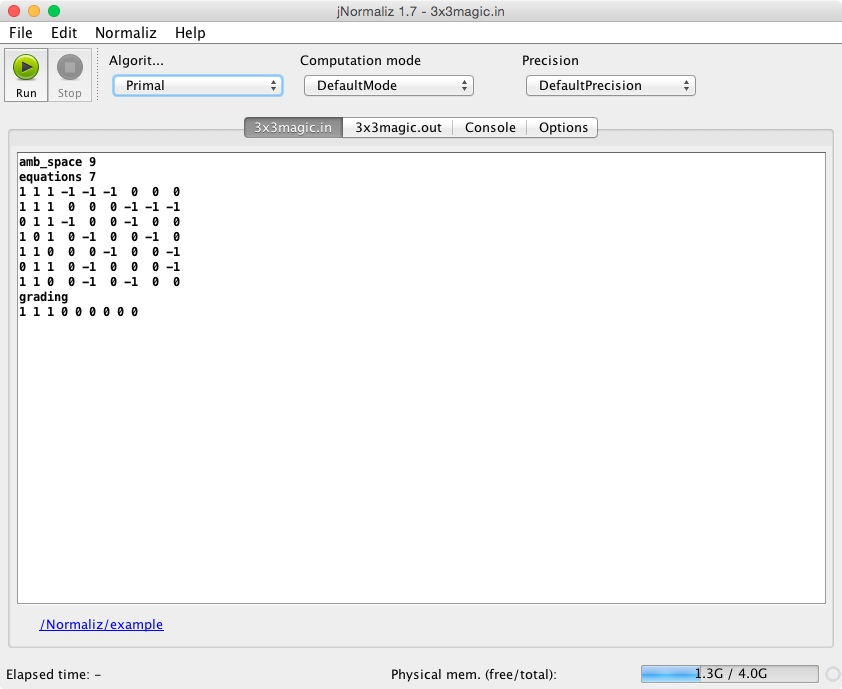
\includegraphics[width = 80 mm, bb=0 0 690 560]{jNormaliz.jpg}\\%width = 80 mm, bb=0 0 689 430
	\caption{jNormaliz}\label{new}
\end{figure}
In the jNormaliz file dialogue choose one of the input files
in the subdirectory \ttt{example}, say \ttt{small.in}, and
press \ttt{Run}. In the console window you can watch Normaliz
at work. Finally inspect the output window for the results.

The menus and dialogues of jNormaliz are self explanatory, but you
can also consult the documentation \cite{AI} via the help menu.

Moreover, one can, and often will, run Normaliz from the
command line. This is fully explained in Section \ref{options}. At this point it is enough to call Normaliz by typing
\begin{Verbatim}
normaliz -c <project>
\end{Verbatim}
where \ttt{<project>} denotes for the project to be computed. Normaliz will load the file \ttt{project.in}. The option \verb|-c| makes Normaliz to write a progress report on the terminal. Normaliz writes its results to \verb|<project>.out|.

Note that you may have to prefix  \ttt{normaliz} by a path name, and \ttt{<project>} must contain a path to the input file if it is not in the current directory. Suppose the Normaliz directory is the current directory and we are using a Linux or Mac system. Then
\begin{Verbatim}
./normaliz -c example/small
\end{Verbatim}
will run \ttt{small.in} from the directory \ttt{example}. On Windows we must change this to
\begin{Verbatim}
.\normaliz -c example\small
\end{Verbatim}

The commands given above will run Normaliz with the full parallelization that your system can deliver. For the very small examples in this tutorial you may want to add \ttt{-x=1} to suppress parallelization.

As long as you don't specify a computation goal on the command line or in the input file, Normaliz will use the \emph{default computation goals}:
\begin{verbatim}
HilbertBasis
HilbertSeries
ClassGroup
\end{verbatim}
The computation of the Hilbert series requires the explicit or implicit definition of a grading. Normaliz does only complain that a computation goal cannot be reached if the goal has been set explicitly. For example, if you say \verb|HilbertSeries| and there is no grading, an exception will be thrown and Normaliz terminates.

Normaliz will always print the results that are obtained on the way to the computation goals and do not require extra effort.

Appendix \ref{Console} helps you to read the console output that you have demanded by the option \verb|-c|.
\subsection{A cone in dimension $2$}\label{cone_ex}

We want to investigate the cone $C=\RR_+(2,1)+\RR_+(1,3)\subset \RR^2$:
\begin{center}
	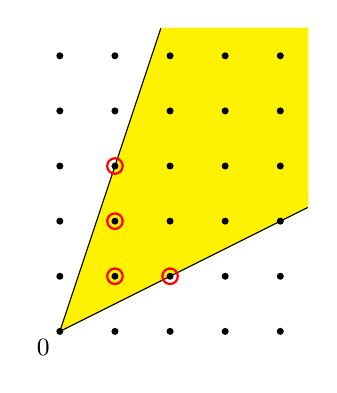
\begin{tikzpicture}[scale=0.7]
	\filldraw[yellow] (0,0) -- (1.833,5.5) -- (4.5,5.5) -- (4.5,2.25) -- cycle;
	\draw (0,0) -- (1.833,5.5);
	\draw (0,0) -- (4.5,2.25) node at (-0.3,-0.3){\small $0$};
	\foreach \x in {0,...,4}
	\foreach \y in {0,...,5}
	{
		\filldraw[fill=black] (\x,\y)  circle (1.5pt);
	}
	\draw[red,thick] (1,1) circle (4pt);
	\draw[red,thick] (1,2) circle (4pt);
	\draw[red,thick] (1,3) circle (4pt);
	\draw[red,thick] (2,1) circle (4pt);
	\end{tikzpicture}
\end{center}

This cone is defined in the input file \verb|2cone.in|:
\begin{Verbatim}
amb_space 2
cone 2
2 1
1 3
\end{Verbatim}
The input tells Normaliz that the ambient space is $\RR^2$, and then a cone with 2 generators is defined, namely the cone $C$ from above.

The figure indicates the Hilbert basis, and this is our first computation goal.

\subsubsection{The Hilbert basis}
In order to compute the Hilbert basis, we run Normaliz from jNormaliz or by
\begin{Verbatim}
./normaliz -c example/2cone	
\end{Verbatim}
and inspect the output file:
\begin{Verbatim}
4 Hilbert basis elements
2 extreme rays
2 support hyperplanes
\end{Verbatim}
Self explanatory so far.
\begin{Verbatim}
embedding dimension = 2
rank = 2 (maximal)
external index = 1
internal index = 5
original monoid is not integrally closed
\end{Verbatim}
The embedding dimension is the dimension of the space in which the computation is done. The rank is the rank of the lattice $\EE$ (notation as in Section \ref{Term}). In fact, in our example $\EE=\ZZ^2$, and therefore has rank $2$.

For subgroups $G\subset U\subset \ZZ^d$ we denote the order of the torsion subgroup of $U/G$ by the \emph{index} of $G$ in $U$. The \emph{external index} is the index of the lattice $\EE$ in $\ZZ^d$. In our case $\EE=\ZZ^d$, and therefore the external index is $1$. Note: the external index is $1$ exactly when $\EE$ is a direct summand of $\ZZ^d$.

For this example and many others the \emph{original monoid} is well defined: the generators of the cone used as input are contained in $\EE$. (This need not be the case if $\EE$ is a proper sublattice of $\ZZ^d$, and we let the original monoid undefined in inhomogeneous computations.) Let $G$ be the subgroup generated by the original monoid. The \emph{internal index} is the index of $G$ in $\EE$.

The original monoid is integrally closed if and only if the it contains the Hilbert basis, and this is evidently false for our example. We go on.

\begin{Verbatim}
size of triangulation   = 1
resulting sum of |det|s = 5
\end{Verbatim}
The primal algorithm of Normaliz relies on a (partial) triangulation. In our case the triangulation consists of a single simplicial cone, and (the absolute value of) its determinant is~$5$.
\begin{Verbatim}
No implicit grading found
\end{Verbatim}
If you do not define a grading explicitly, Normaliz tries to find one itself: It is defined if and only if there is a linear form $\gamma$ on $\EE$ under which all extreme rays of the efficient cone $\CC$ have value $1$, and if so, $\gamma$ is the implicit grading. Such does not exist in our case.

The last information before we come to the vector lists:
\begin{Verbatim}
rank of class group = 0
finite cyclic summands:
5: 1  
\end{Verbatim}
The class group of the monoid $M$ has rank $0$, in other words, it is finite. It has one finite cyclic summand of order $5$.

This is the first instance of a multiset of integers displayed as a sequence of pairs 
\begin{quote}
	\verb|<n>: <m>|
\end{quote} 
Such an entry says: the multiset contains the number \verb|<n>| with multiplicity \verb|<m>.| 


Now we look at the vector lists (typeset in two columns to save space):
\begin{Verbatim}
4 Hilbert basis elements:       2 extreme rays:
1 1                             1 3
1 2                             2 1
1 3
2 1                             2 support hyperplanes:
                                -1  2
                                 3 -1
\end{Verbatim}

The support hyperplanes are given by the linear forms (or inner normal vectors):
\begin{align*}
	-x_1+2x_2&\ge 0,\\
	3x_1-x_2&\ge 0.
\end{align*}

If the order is not fixed for some reason, Normaliz sorts vector lists as follows : (1) by degree if a grading exists and the application makes sense, (2) lexicographically.


\subsubsection{The cone by inequalities}\label{ineq_ex}

Instead by generators, we can define the cone by the inequalities just computed (\verb|2cone_ineq.in|):
\begin{Verbatim}
amb_space 2
inequalities 2
-1  2
3 -1
\end{Verbatim}
A matrix of input type \verb|inequalities| contains \emph{homogeneous} inequalities.

We get the same result as with \verb|2cone.in| except that the data depending on the original monoid cannot be computed: the internal index and the information on the original monoid are missing since there is no original monoid.

\subsubsection{The interior}\label{strict_ex}
Now we want to compute the lattice points in the interior of our cone. If the cone $C$ is given by the inequalities $\lambda_i(x)\ge0$ (within $\aff(C)$), then the interior is given by the inequalities $\lambda_i(x)>0$. Since we are interested in lattice points, we work with the inequalities $\lambda_i(x)\ge 1$.


The input file \verb|2cone_int.in| says
\begin{Verbatim}
amb_space 2
strict_inequalities 2
-1  2
3 -1
\end{Verbatim}
The strict inequalities encode the conditions
\begin{align*}
	-x_1+2x_2&\ge 1,\\
	3x_1-x_2&\ge 1.
\end{align*}
This is our first example of inhomogeneous input.
\begin{center}
	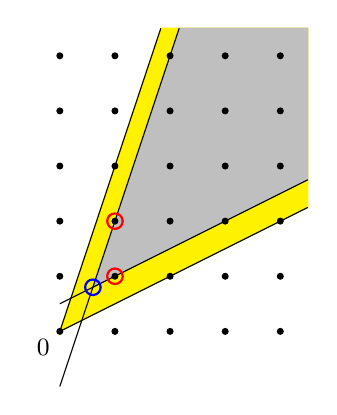
\begin{tikzpicture}[scale=0.7]
	\filldraw[yellow] (0,0) -- (1.833,5.5) -- (4.5,5.5) -- (4.5,2.25) -- cycle;
	\filldraw[lightgray] (0.6,0.8) -- (2.166,5.5) --(4.5,5.5) --  (4.5,2.75) -- cycle;
	\draw (0,0) -- (1.833,5.5);
	\draw (0,0) -- (4.5,2.25) node at (-0.3,-0.3){\small $0$};
	\draw (0,-1) -- (2.166,5.5);
	\draw (0,0.5) -- (4.5,2.75);
	\foreach \x in {0,...,4}
	\foreach \y in {0,...,5}
	{
		\filldraw[fill=black] (\x,\y)  circle (1.5pt);
	}
	\draw[red,thick] (1,1) circle (4pt);
	\draw[red,thick] (1,2) circle (4pt);
	\draw[blue,thick] (0.6,0.8) circle (4pt);
	\end{tikzpicture}
\end{center}

Normaliz homogenizes inhomogeneous computations by introducing an auxiliary homogenizing coordinate $x_{d+1}$. The polyhedron is obtained by intersecting the homogenized cone with the hyperplane $x_{d+1}=1$. The recession cone is the intersection with the hyperplane $x_{d+1}=0$. The recession monoid is the monoid of lattice points in the recession cone, and the set of lattice points in the polyhedron is represented by its system of module generators over the recession monoid.

Note that the homogenizing coordinate serves as the denominator for rational vectors. In our example the recession cone is our old friend that we have already computed, and therefore we need not comment on it.

\begin{Verbatim}
2 module generators
4 Hilbert basis elements of recession monoid
1 vertices of polyhedron
2 extreme rays of recession cone
2 support hyperplanes of polyhedron

embedding dimension = 3
affine dimension of the polyhedron = 2 (maximal)
rank of recession monoid = 2
\end{Verbatim}
The only surprise may be the embedding dimension: Normaliz always takes the dimension of the space in which the computation is done. It is the number of components of the output vectors. Because of the homogenization it has increased by $1$.
\begin{Verbatim}
size of triangulation   = 1
resulting sum of |det|s = 25
\end{Verbatim}
In this case the homogenized cone has stayed simplicial, but the determinant has changed.
\begin{Verbatim}
dehomogenization:
0 0 1 
\end{Verbatim}
The dehomogenization is the linear form $\delta$ on the homogenized space that defines the hyperplanes from which we get the polyhedron and the recession cone by the equations $\delta(x)=1$ and $\delta(x)=0$, respectively. It is listed since one can also work with a user defined dehomogenization.
\begin{Verbatim}
module rank = 1
\end{Verbatim}
This is the rank of the module of lattice points in the polyhedron over the recession monoid. In our case the module is an ideal, and so the rank is $1$.

The output of inhomogeneous computations is always given in homogenized form. The last coordinate is the value of the dehomogenization on the listed vectors, $1$ on the module generators, $0$ on the vectors in the recession monoid:
\begin{Verbatim}
2 module generators:          4 Hilbert basis elements of recession monoid:
1 1 1                         1 1 0
1 2 1                         1 2 0
                              1 3 0
                              2 1 0
\end{Verbatim}
The module generators are $(1,1)$ and $(1,2)$.
\begin{Verbatim}
1 vertices of polyhedron:
3 4 5
\end{Verbatim}
Indeed, the polyhedron has a single vertex, namely $(3/5,4/5)$.
\begin{Verbatim}
2 extreme rays of recession cone:     2 support hyperplanes of polyhedron:
1 3 0                                 -1  2 -1
2 1 0                                  3 -1 -1
\end{Verbatim}
The support hyperplanes are exactly those that we have used to define the polyhedron. This is obvious in our example, but need not always be true since one or more of the defining input hyperplanes may be superfluous.


\subsection{A lattice polytope}\label{lattice_polytope}\label{polytope_ex}

The file \ttt{polytope.in} contains

\begin{Verbatim}
amb_space 4
polytope 4
0 0 0
2 0 0
0 3 0
0 0 5
\end{Verbatim}
\vspace*{-4.5cm}
\hspace*{9cm}
\tikzset{facet style/.style={opacity=1.0,very thick,line,join=round}}
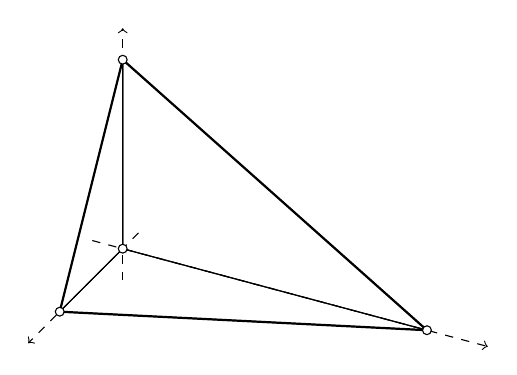
\begin{tikzpicture}[x  = {(-0.5cm,-0.5cm)},
y  = {(0.9659cm,-0.25882cm)},
z  = {(0cm,1cm)},
scale = 0.8]
\draw [->,dashed] (-0.5, 0, 0) -- (3.0,0,0);

\draw [->,dashed] (0, -0.5, 0) -- (0,6.0,0);

\draw [->,dashed] (0, 0, -0.5) -- (0,0,3.5);

\draw[thin] (0,0,0) -- (2,0,0) -- (0,5,0) -- cycle;
\draw[thin] (0,0,0) -- (2,0,0) -- (0,0,3) -- cycle;
\draw[thin] (0,0,0) -- (0,5,0) -- (0,0,3) -- cycle;
\draw[thick] (2,0,0) -- (0,5,0) -- (0,0,3) -- cycle;

\filldraw[fill=white] (0,0,0) circle (2pt);
\filldraw[fill=white] (2,0,0) circle (2pt);
\filldraw[fill=white] (0,5,0) circle (2pt);
\filldraw[fill=white] (0,0,3) circle (2pt);
\end{tikzpicture}


The Ehrhart monoid of the integral polytope with the $4$
vertices
$$
(0,0,0)\,,\quad (2,0,0)\,,\quad (0,3,0)\quad\text{ and }\quad (0,0,5)
$$
in $\RR^3$ is to be computed. The generators of the Ehrhart monoid are obtained by attaching a further coordinate $1$ to the vertices, and this explains \verb|amb_space 4|. In fact, the input type \verb|polytope| is nothing but a convenient (perhaps superfluous)  version of
\begin{Verbatim}
amb_space 4
cone 4
0 0 0 1
2 0 0 1
0 3 0 1
0 0 5 1
\end{Verbatim}

Running \ttt{normaliz} produces the file \ttt{polytope.out}:
\begin{Verbatim}
19 Hilbert basis elements
18 Hilbert basis elements of degree 1
4 extreme rays
4 support hyperplanes

embedding dimension = 4
rank = 4 (maximal)
external index = 1
internal index = 30
original monoid is not integrally closed
\end{Verbatim}
Perhaps a surprise: the lattice points of the polytope do not yield all Hilbert basis elements. 
\begin{Verbatim}
size of triangulation   = 1
resulting sum of |det|s = 30
\end{Verbatim}
Nothing really new so far. But now Normaliz finds a grading given by the last coordinate.  See \ref{grading} below for general information on gradings.
\begin{Verbatim}
grading:
0 0 0 1 

degrees of extreme rays:
1: 4
\end{Verbatim}
Again we encounter the notation \verb|<n>: <m>|: we have $4$ extreme rays, all of degree $1$.
\begin{Verbatim}
Hilbert basis elements are not of degree 1
\end{Verbatim}
Perhaps a surprise: the polytope is not integrally closed as defined in \cite{BG}. Now we see the enumerative data defined by the grading:
\begin{Verbatim}
multiplicity = 30

Hilbert series:
1 14 15 
denominator with 4 factors:
1: 4  

degree of Hilbert Series as rational function = -2

Hilbert polynomial:
1 4 8 5 
with common denominator = 1
\end{Verbatim}
The polytope has $\ZZ^3$-normalized volume $30$ as indicated by the multiplicity. The Hilbert (or Ehrhart) function counts the lattice points in $kP$, $k\in\ZZ_+$. The corresponding generating function is a
rational function $H(t)$. For our polytope it is
$$
\frac{1+14t+15t^2}{(1-t)^4}.
$$
The denominator is given in multiset notation: \verb|1: 4| say that the factor $(1-t^1)$ occurs with multiplicity $4$.

The Ehrhart polynomial (again we use a more general term in
the output file) of the polytope is
$$
p(k)=1+4k+8k^2+5k^3\,.
$$
In our case it has integral coefficients, a rare exception. Therefore one usually needs a denominator.

Everything that follows has already been explained.
\begin{Verbatim}

rank of class group = 0
finite cyclic summands:
30: 1  

***********************************************************************

18 Hilbert basis elements of degree 1:
0 0 0 1
...
2 0 0 1

1 further Hilbert basis elements of higher degree:
1 2 4 2

4 extreme rays:                 4 support hyperplanes:
0 0 0 1                         -15 -10 -6 30
0 0 5 1                         0   0  1  0
0 3 0 1                         0   1  0  0
2 0 0 1                         1   0  0  0
\end{Verbatim}

The support hyperplanes give us a description of the polytope
by inequalities: it is the solution of the system of the $4$
inequalities
$$ x_3\ge0\,,\quad
x_2\ge0\,,\quad x_1\ge0\quad\text{ and }\quad
15x_1+10x_2+6x_3\le30\,.
$$

\subsubsection{Only the lattice points}

Suppose we want to compute only the lattice points in our polytope. In the language of graded monoids these are the degree $1$ elements, and so we add \verb|Deg1Elements| to our input file (\verb|polytope_deg1.in|):
\begin{Verbatim}
amb_space 4
polytope 4
0 0 0
2 0 0
0 3 0
0 0 5
Deg1Elements
/* This is our first explicit computation goal*/
\end{Verbatim}
We have used this opportunity to include a comment in the input file.

We lose all information on the Hilbert series, and from the Hilbert basis we only retain the degree $1$ elements.

\subsection{A rational polytope}\label{rational}

Normaliz has no special input type for rational polytopes.
In order to process them one uses the type \verb|cone| together with a
grading. Suppose the polytope is given by vertices
$$
v_i=(r_{i1},\dots,r_{id}),\qquad i=1,\dots,m,\ r_{ij}\in\QQ.
$$
\begin{center}
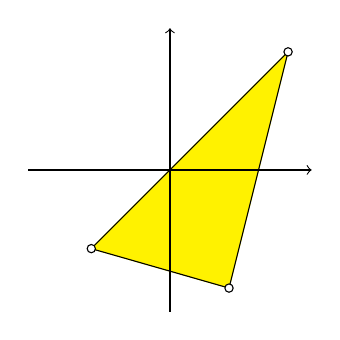
\begin{tikzpicture}[scale=3.0]
\filldraw[yellow] (0.5,0.5) -- (-0.333,-0.333) -- (0.25,-0.5) -- cycle;	
\draw (0.5,0.5) -- (-0.333,-0.333) -- (0.25,-0.5) -- cycle;	
\draw[->] (0,-0.6) --(0,0.6);
\draw[-> ] (-0.6,0) -- (0.6,0);
\filldraw[fill=white] (0.5,0.5) circle (0.5pt);
\filldraw[fill=white] (-0.333,-0.333) circle (0.5pt);
\filldraw[fill=white] (0.25,-0.5) circle (0.5pt);
\end{tikzpicture}
\end{center}
Then we write $v_i$ with a common denominator:
$$
v_i=\biggl(\frac{p_{i1}}{q_i},\dots,\frac{p_{id}}{q_i}\biggr),
\quad p_{ij},q_i\in\ZZ,\ q_i>0.
$$
The generator matrix is given by the rows
$$
\widetilde v_i=(p_{i1},\dots,p_{id},q_i),\quad i=1,\dots,m.
$$
We must add a grading since Normaliz cannot recognize it
without help (unless all the $q_i$ are equal to $1$). The grading
linear form has coordinates $(0,\dots,0,1)$.

We want to investigate the Ehrhart series of the triangle $P$
with vertices
$$
(1/2,1/2),\ (-1/3,-1/3),\ (1/4,-1/2).
$$
For this example the procedure above yields the input file \ttt{rational.in}:

\begin{Verbatim}
amb_space 3
cone 3
1 1 2
-1 -1 3
1 -2 4
grading
unit_vector 3
HilbertSeries
\end{Verbatim}
This is the first time that the we used the shortcut \verb|unit_vector <n>| which represents the $n$-th unit vector $e_n\in\RR^d$ and is only allowed for input types which require a single vector.

From the output file we only list the data of the Ehrhart series.
\begin{Verbatim}
multiplicity = 5/8

Hilbert series:
1 0 0 3 2 -1 2 2 1 1 1 1 2 
denominator with 3 factors:
1: 1  2: 1  12: 1  

degree of Hilbert Series as rational function = -3

Hilbert series with cyclotomic denominator:
-1 -1 -1 -3 -4 -3 -2 
cyclotomic denominator:
1: 3  2: 2  3: 1  4: 1  

Hilbert quasi-polynomial of period 12:
0:   48 28 15			7:   23 22 15
1:   11 22 15			8:   16 28 15
2:  -20 28 15			9:   27 22 15
3:   39 22 15			10:   -4 28 15
4:   32 28 15			11:    7 22 15
5:   -5 22 15			with common denominator = 48
6:   12 28 15
\end{Verbatim}
The multiplicity is a rational number. Since in dimension $2$
the normalized area (of full-dimensional polytopes) is twice
the Euclidean area, we see that $P$ has Euclidean area $5/16$.

Unlike in the case of a lattice polytope, there is no canonical choice of the denominator of the Ehrhart series. Normaliz gives it in $2$ forms. In the first form the numerator polynomial is
$$
1+3t^3+2t^4-t^5+2t^6+2t^7+t^8+t^9+t^{10}+t^{11}+2t^{12}
$$
and the denominator is
$$
(1-t)(1-t^2)(1-t^{12}).
$$
As a rational function, $H(t)$ has degree $-3$. This implies
that $3P$ is the smallest integral multiple of $P$ that
contains a lattice point in its interior.

Normaliz gives also a representation as a quotient of coprime
polynomials with the denominator factored into cyclotomic
polynomials. In this case
we have
$$
H(t)=-\frac{1+t+t^2+t^3+4t^4+3t^5+2t^6}{\zeta_1^3\zeta_2^2\zeta_3\zeta_4}
$$
where $\zeta_i$ is the $i$-th cyclotomic polynomial
($\zeta_1=t-1$, $\zeta_2=t+1$, $\zeta_3=t^2+t+1$,
$\zeta_4=t^2+1$).

Normaliz transforms the representation with cyclotomic
denominator into one with denominator of type
$(1-t^{e_1})\cdots(1-t^{e_r})$, $r=\textup{rank}$, by choosing
$e_r$ as the least common multiple of all the orders of the
cyclotomic polynomials appearing, $e_{r-1}$ as the lcm of those
orders that have multiplicity $\ge 2$ etc.

There are other ways to form a suitable denominator with $3$
factors $1-t^e$, for example
$g(t)=(1-t^2)(1-t^3)(1-t^4)=-\zeta_1^3\zeta_2^2\zeta_3\zeta_4$.
Of course, $g(t)$ is the optimal choice in this case. However,
$P$ is a simplex, and in general such optimal choice may not
exist. We will explain the reason for our standardization
below.

Let $p(k)$ be the number of lattice points in $kP$. Then $p(k)$
is a quasipolynomial:
$$
p(k)=p_0(k)+p_1(k)k+\dots+p_{r-1}(k)k^{r-1},
$$
where the coefficients depend on $k$, but only to the extent
that they are periodic of a certain period $\pi\in\NN$. In our
case $\pi=12$ (the lcm of the orders of the cyclotomic
polynomials).

The table giving the quasipolynomial is to be read as follows:
The first column denotes the residue class $j$ modulo the
period and the corresponding line lists the coefficients
$p_i(j)$ in ascending order of $i$, multiplied by the common
denominator. So
$$
p(k)=1+\frac{7}{12}k+\frac{5}{16}k^2, \qquad k\equiv 0\pod{12},
$$
etc. The leading coefficient is the same for all residue
classes and equals the Euclidean volume.

Our choice of denominator for the Hilbert series is motivated
by the following fact: $e_i$ is the common period of the
coefficients $p_{r-i},\dots,p_{r-1}$. The user should prove
this fact or at least verify it by several examples.

\emph{Warning}: It is tempting, but not a good idea to define the poyltope by the input type \verb|vertices|. It would Normaliz compute the lattice points in the polytope, but not in the cone over the polytope, and we need these to determine the Ehrhart series.

\subsubsection{The rational polytope by inequalities}\label{rat_ineq}

We extract the support hyperplanes of our polytope from the output file and use them as input (\verb|poly_ineq.in|):
\begin{Verbatim}
amb_space 3
inequalities 3
-8  2 3
1 -1 0
2  7 3
grading
unit_vector 3
HilbertSeries
\end{Verbatim}

These data tell us that the polytope, as a subset of $\RR^2$, is defined by the inequalities
\begin{align*}
	-8x_1+2x_2+3&\ge0,\\
	x_1-x_2+0&\ge0,\\
	2x_1+7x_2+3&\ge 0.
\end{align*}
These inequalities are inhomogeneous, but we are using the homogeneous input type \verb|inequalities| which amounts to introducing the grading variable $x_3$, as we have done it for the generators.

Why don't we define it by the ``natural'' inhomogeneous inequalities using \verb|inhom_inequalities|? We could do it, but then only the polytope itself would be the object of computation, and we would have no access to the Ehrhart series. We could just compute the lattice points in the polytope. (Try it.)


\subsection{Magic squares}\label{eq_ex}

Suppose that you are interested in the following `type of `square''
\begin{center}
	\begin{tabular}{|l|l|l|}
		\hline
		$x_1$ & $x_2$ & $x_3$\\
		\hline
		$x_4$ & $x_5$ & $x_6$\\
		\hline
		$x_7$ & $x_8$ & $x_9$\\
		\hline
	\end{tabular}
\end{center}
and the problem is to find nonnegative values for $x_1,\dots,x_9$
such that the 3 numbers in all rows, all columns, and both
diagonals sum to the same constant $\mathcal{M}$. Sometimes
such squares are called \emph{magic} and $\mathcal M$ is the
\emph{magic constant}. This leads to a linear system of
equations
\begin{align*}
	& x_1+x_2+x_3=x_4+x_5+x_6;\\
	& x_1+x_2+x_3=x_7+x_8+x_9;\\
	& x_1+x_2+x_3=x_1+x_4+x_7;\\
	& x_1+x_2+x_3=x_2+x_5+x_8;\\
	& x_1+x_2+x_3=x_3+x_6+x_9;\\
	& x_1+x_2+x_3=x_1+x_5+x_9;\\
	& x_1+x_2+x_3=x_3+x_5+x_7.\\
\end{align*}
This system is encoded in the file
\ttt{3x3magic.in}:
\begin{Verbatim}
amb_space 9
equations 7
1 1 1 -1 -1 -1  0  0  0
1 1 1  0  0  0 -1 -1 -1
0 1 1 -1  0  0 -1  0  0
1 0 1  0 -1  0  0 -1  0
1 1 0  0  0 -1  0  0 -1
0 1 1  0 -1  0  0  0 -1
1 1 0  0 -1  0 -1  0  0
grading
1 1 1 0 0 0 0 0 0
\end{Verbatim} 
The input type \verb|equations| represents \emph{homogeneous} equations. The first equation reads
$$
x_1+x_2+x_3-x_4-x_5-x_6=0,
$$
and the other equations are to be interpreted analogously. The magic constant is a natural choice for the grading. 

It seems that we have forgotten to define the cone. This may indeed be the case, but doesn't matter: if there is no input type that defines a cone, Normaliz chooses the positive orthant, and this is exactly what we want in this case.

The output file contains the following:

\begin{Verbatim}
5 Hilbert basis elements
5 Hilbert basis elements of degree 1
4 extreme rays
4 support hyperplanes

embedding dimension = 9
rank = 3
external index = 1

size of triangulation   = 2
resulting sum of |det|s = 4

grading:
1 1 1 0 0 0 0 0 0 
with denominator = 3
\end{Verbatim}
The input degree is the magic constant. However, as the
denominator $3$ shows, the magic constant is always divisible
by $3$, and therefore the effective degree is $\mathcal M/3$.
This degree is used for the multiplicity and the Hilbert
series.
\begin{Verbatim}
degrees of extreme rays:
1: 4  

Hilbert basis elements are of degree 1
\end{Verbatim}
This was not to be expected (and is no longer true for $4\times 4$ squares).
\begin{Verbatim}
multiplicity = 4

Hilbert series:
1 2 1 
denominator with 3 factors:
1: 3  

degree of Hilbert Series as rational function = -1

Hilbert polynomial:
1 2 2 
with common denominator = 1
\end{Verbatim}
The Hilbert series is
$$
\frac{1+2t+t^2}{(1-t)^3}.
$$
The Hilbert polynomial is
$$
P(k)=1+2k+2k^2,
$$
and after substituting $\mathcal M/3$ for $k$ we obtain the
number of magic squares of magic constant $\mathcal M$, provided $3$ divides $\mathcal M$. (If $3\nmid \mathcal M$, there is no magic square of magic constant $\mathcal M$.)
\begin{Verbatim}
rank of class group = 1
finite cyclic summands:
2: 2  
\end{Verbatim}
So the class group is $\ZZ\oplus (\ZZ/2\ZZ)^2$.
\begin{Verbatim}
5 Hilbert basis elements of degree 1:
0 2 1 2 1 0 1 0 2
1 0 2 2 1 0 0 2 1
1 1 1 1 1 1 1 1 1
1 2 0 0 1 2 2 0 1
2 0 1 0 1 2 1 2 0

0 further Hilbert basis elements of higher degree:
\end{Verbatim}
The $5$ elements of the Hilbert basis represent the magic
squares
\begin{center}
	\begin{tabular}{|l|l|l|}
		\hline
		2 & 0 & 1\\
		\hline
		0 & 1 & 2\\
		\hline
		1 & 2 & 0\\
		\hline
	\end{tabular}
	\hspace{10mm}
	\begin{tabular}{|l|l|l|}
		\hline
		1 & 0 & 2\\
		\hline
		2 & 1 & 0\\
		\hline
		0 & 2 & 1\\
		\hline
	\end{tabular}
	\hspace{10mm}
	\begin{tabular}{|l|l|l|}
		\hline
		1 & 1 & 1\\
		\hline
		1 & 1 & 1\\
		\hline
		1 & 1 & 1\\
		\hline
	\end{tabular}
	\hspace{10mm}
	\begin{tabular}{|l|l|l|}
		\hline
		1 & 2 & 0\\
		\hline
		0 & 1 & 2\\
		\hline
		2 & 0 & 1\\
		\hline
	\end{tabular}
	\hspace{10mm}
	\begin{tabular}{|l|l|l|}
		\hline
		0 & 2 & 1\\
		\hline
		2 & 1 & 0\\
		\hline
		1 & 0 & 2\\
		\hline
	\end{tabular}	
\end{center}
All other solutions are linear combinations of these squares
with nonnegative integer coefficients.
One of these $5$ squares is clearly in the interior:
\begin{Verbatim}
4 extreme rays:                  4 support hyperplanes:
0 2 1 2 1 0 1 0 2                -2 -1 0 0  4 0 0 0 0
1 0 2 2 1 0 0 2 1                0 -1 0 0  2 0 0 0 0
1 2 0 0 1 2 2 0 1                0  1 0 0  0 0 0 0 0
2 0 1 0 1 2 1 2 0                2  1 0 0 -2 0 0 0 0
\end{Verbatim}
These $4$ support hyperplanes cut out the cone generated by the magic squares from the linear subspace they generate. Only one is reproduced as a sign inequality. This is due to the fact that the linear subspace has submaximal dimension and there is no unique lifting of linear forms to the full space.
\begin{Verbatim}
6 equations:                    3 basis elements of lattice:
1 0 0 0 0  1 -2 -1  1           1 0 -1 -2 0  2  1  0 -1
0 1 0 0 0  1 -2  0  0           0 1 -1 -1 0  1  1 -1  0
0 0 1 0 0  1 -1 -1  0           0 0  3  4 1 -2 -1  2  2
0 0 0 1 0 -1  2  0 -2
0 0 0 0 1 -1  1  0 -1
0 0 0 0 0  3 -4 -1  2
\end{Verbatim}
So one of our equations has turned out to be superfluous (why?). Note that also the equations are not reproduced exactly. Finally, Normaliz lists a basis of the efficient lattice $\EE$  generated by the magic squares.

\subsubsection{With even corners}\label{magiceven}\label{cong_ex}

We change our definition of magic square by requiring that the
entries in the $4$ corners are all even. Then we have to
augment the input file by the following (\ttt{3x3magiceven.in}):
\begin{Verbatim}
congruences 4
1 0 0 0 0 0 0 0 0 2
0 0 1 0 0 0 0 0 0 2
0 0 0 0 0 0 1 0 0 2
0 0 0 0 0 0 0 0 1 2
\end{Verbatim}
The first $9$ entries in each row represent the coefficients of the coordinates in the homogeneous congruences, and the last is the modulus:
$$
x_1\equiv 0\mod 2
$$
is the first congruence etc.

The output changes accordingly:


\begin{Verbatim}
9 Hilbert basis elements
0 Hilbert basis elements of degree 1
4 extreme rays
4 support hyperplanes

embedding dimension = 9
rank = 3
external index = 4

size of triangulation   = 2
resulting sum of |det|s = 8

grading:
1 1 1 0 0 0 0 0 0 
with denominator = 3

degrees of extreme rays:
2: 4  

multiplicity = 1

Hilbert series:
1 -1 3 1 
denominator with 3 factors:
1: 1  2: 2  

degree of Hilbert Series as rational function = -2

Hilbert series with cyclotomic denominator:
-1 1 -3 -1 
cyclotomic denominator:
1: 3  2: 2  

Hilbert quasi-polynomial of period 2:
0:   2 2 1
1:  -1 0 1
with common denominator = 2
\end{Verbatim}
After the extensive discussion in Section \ref{rational} it should be easy for you to write down the Hilbert series and the Hilbert quasipolynomial. (But keep in mind that the grading has a denominator.)
\begin{Verbatim}
rank of class group = 1
finite cyclic summands:
4: 2  

***********************************************************************

0 Hilbert basis elements of degree 1:

9 further Hilbert basis elements of higher degree:
...

4 extreme rays:
0 4 2 4 2 0 2 0 4
2 0 4 4 2 0 0 4 2
2 4 0 0 2 4 4 0 2
4 0 2 0 2 4 2 4 0
\end{Verbatim}
We have listed the extreme rays since they have changed after the introduction of the congruences, although the cone has not changed. The reason is that Normaliz always chooses the extreme rays from the efficient lattice $\EE$.
\begin{Verbatim}

4 support hyperplanes:
...

6 equations:
...                              3 basis elements of lattice:
                                 2 0 -2 -4 0  4  2 0 -2
2 congruences:                   0 1  2  3 1 -1  0 1  2
1 0 0 0 0 0 0 0 0 2              0 0  6  8 2 -4 -2 4  4
0 1 0 0 1 0 0 0 0 2
\end{Verbatim}
The rank of the lattice has of course not changed, but after the introduction of the congruences the basis has changed.

\subsubsection{The lattice as input}\label{latt_ex}

It is possible to define the lattice by generators. We demonstrate this for the magic squares with even corners. The lattice has just been computed (\verb|3x3magiceven_lat.in|):

\begin{Verbatim}
amb_space 9
lattice 3
2 0 -2 -4 0  4  2 0 -2
0 1  2  3 1 -1  0 1  2
0 0  6  8 2 -4 -2 4  4
grading
1 1 1 0 0 0 0 0 0
\end{Verbatim}
It produces the same output as the version starting from equations and congruences.

\verb|lattice| has a variant that takes the saturation of the sublattice generated by the input vectors (\verb|3x3magic_sat.in|):

\begin{Verbatim}
amb_space 9
saturation 3
2 0 -2 -4 0  4  2 0 -2
0 1  2  3 1 -1  0 1  2
0 0  6  8 2 -4 -2 4  4
grading
1 1 1 0 0 0 0 0 0
\end{Verbatim}
Clearly, we remove the congruences by this choice and arrive at the output of \verb|3x3magic.in|.

\subsection{Decomposition in a numerical semigroup}\label{inhom_eq_ex}

Let $S=\langle 6,10,15\rangle$, the numerical semigroup generated by $6,10,15$. How can $97$ be written as a sum in the generators?\medskip

In other words: we want to find all nonnegative integral solutions to the equation
$$
6x_1+10x_2+15x_3=97
$$

Input (\verb|NumSemi.in|):
\begin{Verbatim}
amb_space 3
inhom_equations 1
6 10 15 -97
\end{Verbatim}

\vspace*{-2.5cm}
\hspace*{6cm}
\tikzset{facet style/.style={opacity=1.0,very thick,line,join=round}}
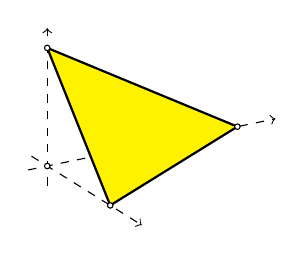
\begin{tikzpicture}[x  = {(0.8cm,-0.5cm)},
y  = {(0.9659cm,0.20cm)},
z  = {(0cm,1cm)},
scale = 0.5]
\draw [->,dashed] (-0.5, 0, 0) -- (3.0,0,0);

\draw [->,dashed] (0, -0.5, 0) -- (0,6.0,0);

\draw [->,dashed] (0, 0, -0.5) -- (0,0,3.5);

%\draw[thin] (0,0,0) -- (2,0,0) -- (0,5,0) -- cycle;
%\draw[thin] (0,0,0) -- (2,0,0) -- (0,0,3) -- cycle;
%\draw[thin] (0,0,0) -- (0,5,0) -- (0,0,3) -- cycle;
\filldraw[color=yellow] (2,0,0) -- (0,5,0) -- (0,0,3) -- cycle;
\draw[thick] (2,0,0) -- (0,5,0) -- (0,0,3) -- cycle;

\filldraw[fill=white] (0,0,0) circle (2pt);
\filldraw[fill=white] (2,0,0) circle (2pt);
\filldraw[fill=white] (0,5,0) circle (2pt);
\filldraw[fill=white] (0,0,3) circle (2pt);
\end{tikzpicture}

\medskip
The equation cuts out a triangle from the positive orthant. 

The set of solutions is a module over the monoid $M$ of solutions of the homogeneous equation $6x_1+10x_2+15x_3=0$. So $M=0$.
\begin{Verbatim}
6 module generators:
2 1 5 1
2 4 3 1
2 7 1 1
7 1 3 1
7 4 1 1
12 1 1 1

0 Hilbert basis elements of recession monoid:
\end{Verbatim}
The last line is as expected, and the $6$ module generators are the goal of the computation.

Normaliz is smart enough to recognize that it must compute the lattice points in a polygon, and does exactly this. You can recognize it in the console output: it contains the line

\begin{Verbatim}
Converting polyhedron to polytope
\end{Verbatim}

\subsection{A job for the dual algorithm}

We increase the size of the magic squares to $5\times 5$. Normaliz can do the same computation as for $3\times 3$ squares, but this will take some minutes. If we are only interested in the Hilbert basis, we should use the dual algorithm for this example. The input file is \ttt{5x5dual.in}:

\begin{Verbatim}
amb_space 25
equations 11
1 1 1 1 1 -1 -1 -1 -1 -1  0  0  0  0  0  0  0  0  0  0  0  0  0  0  0
...
1 1 1 1 0  0  0  0 -1  0  0  0 -1  0  0  0 -1  0  0  0 -1  0  0  0  0
DualMode
grading
1 1 1 1 1 0 0 0 0 0 0 0 0 0 0 0 0 0 0 0 0 0 0 0 0
\end{Verbatim}
The choice of the dual algorithm implies the computation goal \verb|HilbertBasis|. By adding \verb|Deg1Elements| we could restrict the computation to the degree $1$ elements.


The Hilbert basis contains $4828$ elements, too many to be listed here.

If you want to run this example with default computation goals, use the file \verb|5x5_default.in|. It will compute the Hilbert basis and the Hilbert series.

The size $6\times 6$ is out of reach for the Hilbert series, but the Hilbert basis can be computed in dual mode. It takes some hours.

\subsection{A dull polyhedron}\label{inhom_ineq_ex}

We want to compute the polyhedron defined by the inequalities
\begin{align*}
	\xi_2 &\ge -1/2 &\iff 0\xi_1+2\xi_2+1&\ge 0\\
	\xi_2 &\le 3/2 &\iff 0\xi_1-2\xi_2+3&\ge0\\
	\xi_2 &\le \xi_1+3/2&\iff 2\xi_1-2\xi_2+3&\ge0
\end{align*}
They are contained in the input file \verb|InhomIneq.in|:
\begin{Verbatim}
amb_space 2
inhom_inequalities 3
0  2  1
0 -2  3
2 -2  3
grading
unit_vector 1
\end{Verbatim}
The grading says that we want to count points by the first coordinate.
\begin{center}
	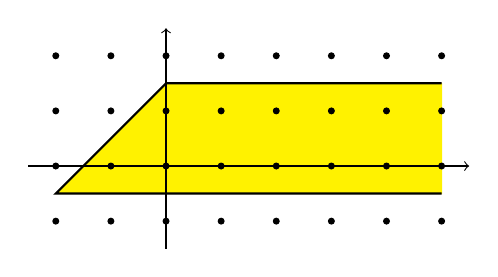
\begin{tikzpicture}[scale=0.7]
	
	\filldraw[yellow] (5,-0.5) -- (-2,-0.5) -- (0,1.5) -- (5,1.5) -- cycle;
	
	\foreach \x in {-2,...,5}
	\foreach \y in {-1,...,2}
	{
		\filldraw[fill=black] (\x,\y)  circle (1.5pt);
	}
	\draw[->] (-2.5,0) -- (5.5,0);
	\draw[->] (0,-1.5) -- (0,2.5);
	\draw[thick] (5,-0.5) -- (-2,-0.5) -- (0,1.5) -- (5,1.5); 
	\end{tikzpicture}
\end{center}

It yields the output
\begin{Verbatim}
2 module generators
1 Hilbert basis elements of recession monoid
2 vertices of polyhedron
1 extreme rays of recession cone
3 support hyperplanes of polyhedron

embedding dimension = 3
affine dimension of the polyhedron = 2 (maximal)
rank of recession monoid = 1

size of triangulation   = 1
resulting sum of |det|s = 8

dehomogenization:
0 0 1 

grading:
1 0 0 
\end{Verbatim}
The interpretation of the grading requires some care in the inhomogeneous case. We have extended the input grading vector by an entry $0$ to match the embedding dimension. For the computation of the degrees of \emph{lattice points} in the ambient space you can either use only the first $2$ coordinates or take the full scalar product of the point in homogenized coordinates and the extended grading vector.

\begin{Verbatim}
module rank = 2
multiplicity = 2
\end{Verbatim}
The module rank is $2$ in this case since we have two ``layers'' in the solution module that are parallel to the recession monoid. This is of course also reflected in the Hilbert series.
\begin{Verbatim}
Hilbert series:
1 1 
denominator with 1 factors:
1: 1  

shift = -1
\end{Verbatim}
We haven't seen a shift yet. It is always printed (necessarily) if the Hilbert series does not start in degree $0$. In our case it starts in degree $-1$ as indicated by the shift $-1$. We thus get the Hilbert series
$$
t^{-1}\,\frac{t+t}{1-t}=\frac{t^{-1}+1}{1-t}.
$$

Note: We used the opposite convention for the shift in Normaliz 2.

Note that the Hilbert (quasi)polynomial is always computed for the unshifted monoid defined by the input data. (This was different in previous versions of Normaliz.) 
\begin{Verbatim}
degree of Hilbert Series as rational function = -1

Hilbert polynomial:
2 
with common denominator = 1

***********************************************************************

2 module generators:
-1 0 1
0 1 1

1 Hilbert basis elements of recession monoid:
1 0 0

2 vertices of polyhedron:
-4 -1 2
0  3 2

1 extreme rays of recession cone:
1 0 0

3 support hyperplanes of polyhedron:
0 -2 3
0  2 1
2 -2 3
\end{Verbatim}

\subsubsection{Defining it by generators}\label{polyh_ex}

If the polyhedron is given by its vertices and the recession cone, we can define it by these data (\verb|InhomIneq_gen.in|):
\begin{Verbatim}
amb_space 2
vertices 2
-4 -1 2
0  3 2
cone 1
1 0
grading
unit_vector 1
\end{Verbatim}
The output is identical to the version starting from the inequalities.

\subsection{The Condorcet paradoxon}\label{Condorcet}

In social choice elections each of the $k$ voters picks a preference order of the $n$ candidates. There are $n!$ such orders.
\medskip 

We say that candidate $A$ \emph{beats} candidate $B$ if the majority of the voters prefers $A$ to $B$. As the Marquis de \emph{Condorcet} (and others) observed, ``beats'' is not transitive, and an election may exhibit the \emph{Condorcet paradoxon}: there is no Condorcet winner. (See \cite{BS} and the references given there for more information.)

We want to find the probability for $k\to\infty$ that there is a Condorcet winner for $n=4$ candidates. The event that $A$ is the Condorcet winner can be expressed by linear inequalities on the election outcome (a point in $24$-space). The wanted probability is the lattice normalized volume of the polytope cut out by the inequalities at $k=1$. The file \verb|Condorcet.in|:

\begin{Verbatim}
amb_space 24
inequalities 3
1 1 1 1 1 1 -1 -1 -1 -1 -1 -1   1  1 -1 -1  1 -1   1  1 -1 -1  1 -1
1 1 1 1 1 1  1  1 -1 -1  1 -1  -1 -1 -1 -1 -1 -1   1  1  1 -1 -1 -1
1 1 1 1 1 1  1  1  1 -1 -1 -1   1  1  1 -1 -1 -1  -1 -1 -1 -1 -1 -1
nonnegative
total_degree
Multiplicity
\end{Verbatim}
The first inequality expresses that $A$ beats $B$, the second and the third say that $A$ beats $C$ and $D$. (So far we do not exclude ties, and they need not be excluded for probabilities as $k\to\infty$.)

In addition to these inequalities we must restrict all variables to nonnegative values, and this is achieved by adding the attribute \verb|nonnegative|. The grading is set by \verb|total_degree|. It replaces the grading vector with $24$ entries $1$. Finally \verb|Multiplicity| sets the computation goal.

From the output file we only mention the quantity we are out for:
\begin{Verbatim}
multiplicity = 1717/8192
\end{Verbatim}
Since there are $4$ candidates, the probability for the existence of a Condorcet winner is $1717/2048$.

\subsubsection{Excluding ties}\label{excluded_ex}

Now we are more ambitious and want to compute the Hilbert series for the Condorcet paradoxon, or more precisely, the number of election outcomes having $A$ as the Condorcet winner depending on the number $k$ of voters. Moreover, as it is customary in social choice theory, we want to exclude ties. The input file changes to \verb|CondorcetSemi.in|:
\begin{Verbatim}
amb_space 24
excluded_faces 3
1 1 1 1 1 1 -1 -1 -1 -1 -1 -1   1  1 -1 -1  1 -1   1  1 -1 -1  1 -1
1 1 1 1 1 1  1  1 -1 -1  1 -1  -1 -1 -1 -1 -1 -1   1  1  1 -1 -1 -1
1 1 1 1 1 1  1  1  1 -1 -1 -1   1  1  1 -1 -1 -1  -1 -1 -1 -1 -1 -1
nonnegative
total_degree
HilbertSeries
\end{Verbatim}
We could omit \verb|HilbertSeries|, and the computation would include the Hilbert basis. The type \verb|excluded_faces| only affects the Hilbert series. In every other respect it is equivalent to \verb|inequalities|.

Please have a look at \verb|CondorcetSemi.out|.

It is justified to ask why we don't use \verb|strict_inequalities| instead of \verb|excluded_faces|. It does of course give the same Hilbert series. If there are many excluded faces, then it is better to use \verb|strict_inequalities|. However, at present NmzIntegrate can only work with \verb|excluded_faces|.

\subsubsection{At least one vote for every preference order}\label{strict_signs_ex}

Suppose we are only interested in elections in which every preference order is chosen by at least one voter. This can be modeled as follows (\verb|Condorcet_one.in|):
\begin{Verbatim}
amb_space 24
inequalities 3
1 1 1 1 1 1 -1 -1 -1 -1 -1 -1   1  1 -1 -1  1 -1   1  1 -1 -1  1 -1
1 1 1 1 1 1  1  1 -1 -1  1 -1  -1 -1 -1 -1 -1 -1   1  1  1 -1 -1 -1
1 1 1 1 1 1  1  1  1 -1 -1 -1   1  1  1 -1 -1 -1  -1 -1 -1 -1 -1 -1
strict_signs
1 1 1 1 1 1 1 1 1 1 1 1 1 1 1 1 1 1 1 1 1 1 1 1
total_degree
HilbertSeries
\end{Verbatim}
The entry $1$ at position $i$ of the vector \verb|strict_signs| imposes the inequality $x_i\ge1$. A $-1$ would impose the inequality $x_i\le -1$, and the entry $0$ imposes no condition on the $i$-th coordinate.

In the output file we see the numerator polynomial of the Hilbert series of \verb|CondorcetSemi.in| in reverse order of coefficients. This is an example of generalized Ehrhart reciprocity; see \cite[Theorem 6.70]{BG}.

If we want the interior of the Condorcet cone, we must use \verb|strict_inequalities| on place of \verb|inequalities| in order to see an example of ``ordinary'' Ehrhart reciprocity.


\subsection{Testing normality}\label{normalization_ex}

We want to test the monoid $A_{4\times 4\times 3}$ defined by $4\times4\times3$ contingency tables for normality (see \cite{BHIKS} for the background). The input file is \ttt{A443.in}:
\begin{Verbatim}
amb_space 40
cone_and_lattice 48
1 0 0 0 0 0 0 0 0 0 0 0 0 0 0 0 1 0 0 0 0 0 0 0 0 0 0 0 1 0 0 0 0 0 0 0 0 0 0 0
...
0 0 0 0 0 0 0 0 0 0 0 0 0 0 0 1 0 0 0 0 0 0 0 0 0 0 0 1 0 0 0 0 0 0 0 0 0 0 0 1
HilbertBasis
\end{Verbatim}
Why \verb|cone_and_lattice|? Well, we want to find out whether the monoid is normal, i.e., whether $M=C(M)\cap\gp(M)$. If $M$ is even integrally closed in $\ZZ^{24}$, then it is certainly integrally closed  in the evidently smaller lattice $\gp(M)$, but the converse does not hold in general, and therefore we work with the lattice generated by the monoid generators.

It turns out that the monoid is indeed normal:
\begin{Verbatim}
original monoid is integrally closed
\end{Verbatim}
Actually the output file reveals that $M$ is even integrally closed in $\ZZ^{24}$: the external index is $1$, and therefore $\gp(M)$ is integrally closed in $\ZZ^{24} $. 

The output files also shows that there is a grading on $\ZZ^{24}$ under which all our generators have degree $1$. We could have seen this ourselves: Every generator has exactly one entry $1$ in the first $16$ coordinates. (This is clear from the construction of $M$.)

A noteworthy detail from the output file:
\begin{Verbatim}
size of partial triangulation   = 48
\end{Verbatim}
It shows that Normaliz uses only a partial triangulation in Hilbert basis computations; see \cite{BHIKS}.

It is no problem to compute the Hilbert series as well if you are interested in it. Simply add \verb|-q| to the command line or remove \verb|HilberBasis| from the input file. Then a full triangulation is needed (size $2,654,272$).

Similar examples are \verb|A543|, \verb|A553| and \verb|A643|. The latter is not normal. Even on a standard PC or laptop, the Hilbert basis computation does not take very long because Normaliz uses only a partial triangulation. The Hilbert series can still be determined, but the computation time will grow considerably since the it requires a full triangulation. See \cite{BIS} for timings.

\subsection{Inhomogeneous congruences}\label{ChinRem}

We want to compute the nonnegative solutions of the simultaneous inhomogeneous congruences
\begin{align*}
	x_1 + 2x_2 &\equiv 3\pod 7,\\
	2x_1 + 2x_2 &\equiv 4\pod{13}
\end{align*}
in two variables. As usual we move the right hand side over to the left. The input file \verb|InhomCong.in| is
\begin{Verbatim}
amb_space 2
inhom_congruences 2
1 2 -3 7
2 2 -4 13
\end{Verbatim}

The first vector list in the output:

\begin{Verbatim}
3 module generators:
0 54 1
1  1 1
80  0 1
\end{Verbatim}
Easy to check: if $(1,1)$ is a solution, then it must generate the module of solutions together with the generators of the intersections with the coordinate axes. Perhaps more difficult to find: 
\begin{Verbatim}
6 Hilbert basis elements of recession monoid:
 0 91 0
 1 38 0
 3 23 0                  1 vertices of polyhedron:
 5  8 0                  0 0 91
12  1 0
91  0 0
\end{Verbatim}
Strange, why not the vertex $(0,0,1)$, representing the origin in $\RR^2$ as well? Well the vertex shown represents an extreme ray in the lattice $\EE$, and $(0,0,1)$ does not belong to $\EE$.
\begin{Verbatim}

2 extreme rays of recession cone:
0 91 0
91  0 0

2 support hyperplanes of polyhedron:
0 1 0
1 0 0

1 congruences:
58 32 1 91
\end{Verbatim}
Normaliz has simplified the system of congruences to a single one.
\begin{Verbatim}
3 basis elements of lattice:
1 0  33
0 1 -32
0 0  91
\end{Verbatim}
Again, don't forget that Normaliz prints a basis of the efficient lattice $\EE$.

\subsubsection{Lattice and offset}\label{offset_ex}

The set of solutions to the inhomogeneous system is an affine lattice in $\RR^2$. The lattice basis of $\EE$ above does not immediately let us write down the set of solutions in the form $w+L_0$ with a subgroup $L_0$, but we can easily transform the basis of $\EE$: just add the first and the second vector to obtain $(1,1,1)$ -- we already know that it belongs to $\EE$ and any element in $\EE$ with last coordinate $1$ would do. Try the file \verb|InhomCongLat.in|:

\begin{Verbatim}
amb_space 2
offset
1 1
lattice 2
32 33
91 91
\end{Verbatim}


\subsubsection{Variation of the signs}\label{sign_ex}

Suppose we want to solve the system of congruences under the condition that both variables are negative (\verb|InhomCongSigns.in|): 

\begin{Verbatim}
amb_space 2
inhom_congruences 2
1 2 -3 7
2 2 -4 13
signs
-1 -1
\end{Verbatim}
The two entries of the sign vector impose the sign conditions $x_1\le 0$ and $x_2\le 0$.

From the output we see that the module generators are more complicated now:
\begin{Verbatim}
4 module generators:
-11   0 1
-4  -7 1
-2 -22 1
0 -37 1
\end{Verbatim}
The Hilbert basis of the recession monoid is simply that of the nonnegative case multiplied by $-1$.

\subsection{Integral closure and Rees algebra of a monomial ideal}\label{Rees}

Next, let us discuss the example \ttt{MonIdeal.in} (typeset in two columns):

\begin{Verbatim}
amb_space 5
rees_algebra 9
1 2 1 2                 1 0 3 4
3 1 1 3                 5 1 0 1
2 5 1 0                 2 4 1 5
0 2 4 3                 2 2 2 4
0 2 3 4
\end{Verbatim}
The input vectors are the exponent vectors of a monomial ideal $I$  in the ring $K[X_1,X_2,X_3,X_4]$. We want to compute the normalization of the Rees algebra of the ideal. In particular we can extract from it the integral closure of the ideal. Since we must introduce an extra variable $T$, we have \verb|amb_space 5|.  

In the Hilbert basis we see the exponent vectors of the $X_i$, namely the unit vectors with last component $0$. The vectors with last component $1$ represent the integral closure $\overline I$  of the ideal. There is a  vector with last component $2$, showing that the integral closure of $I^2$ is larger than~$\overline I^2$.
\begin{Verbatim}
16 Hilbert basis elements:
0 0 0 1 0
...
5 1 0 1 1
6 5 2 2 2

11 generators of integral closure of the ideal:
0 2 3 4
...
5 1 0 1
\end{Verbatim}
This output is the only place where we suppress the homogenizing variable for ``historic'' reasons. If we extract the vectors with last component $1$ from the extreme rays, then we obtain the smallest monomial ideal that has the same integral closure as $I$.
\begin{Verbatim}
10 extreme rays:
0 0 0 1 0
...
5 1 0 1 1
\end{Verbatim}
The support hyperplanes which are not just sign conditions describe primary decompositions of all the ideals $\overline{I^k}$ by valuation ideals. It is not hard to see that none of them can be omitted for large $k$ (for example, see: W. Bruns and G. Restuccia,  Canonical modules of Rees algebras. J. Pure Appl. Algebra 201, 189--203 (2005)).
\begin{Verbatim}
23 support hyperplanes:
0 0 0  0   1
0 ...
6 0 1  3 -13
\end{Verbatim}

\subsubsection{Only the integral closure}

If only the integral closure of the ideal is to be computed, one can choose the input as follows (\verb|IntClMonId.in|):
\begin{Verbatim}
amb_space 4
vertices 9
1 2 1 2 1
...
2 2 2 4 1
cone 4
1 0 0 0
0 1 0 0
0 0 1 0
0 0 0 1
\end{Verbatim}

The generators of the integral closure appear as module generators in the output and the generators of the smallest monomial ideal with this integral closure are the vertices of the polyhedron.

\subsection{Only the convex hull}

Normaliz computes convex hulls as should be very clear by now, and the only purpose of this section is to emphasize that the computation can be restricted to it by setting an explicit computation goal. We choose the input of the preceding section and add the computation goal (\verb|IntClMonIdSupp.in|):

\begin{Verbatim}
amb_space 4
vertices 9
1 2 1 2 1
...
2 2 2 4 1
vertices
cone 4
1 0 0 0
...
0 0 0 1
SupportHyperplanes
\end{Verbatim}

As you can see from the output, the support hyperplanes of the polyhedron are computed as well as the extreme rays.


\subsection{Starting from a binomial ideal}\label{binom_ex}

As an example, we consider the binomial ideal generated by
$$
X_1^2X_2-X_4X_5X_6,\ \ X_1X_4^2-X_3X_5X_6,\ \ X_1X_2X_3-X_5^2X_6.
$$
We want to find an embedding of the toric ring it defines and
the normalization of the toric ring. The input vectors are obtained as the differences of the two exponent vectors in the binomials. So the input ideal \verb+lattice_ideal.in+ is
\begin{Verbatim}
amb_space 6
lattice_ideal 3
2 1  0 -1 -1  -1
1 0 -1  2 -1  -1
1 1  1  0 -2  -1
\end{Verbatim}
In order to avoid special input rules for this case in which our object is not defined as a subset of an ambient space, but as a quotient of type \emph{generators/relations}, we abuse the name \verb|amb_space|: it determines the space in which the input vectors live.

We get the output
\begin{Verbatim}
6 original generators of the toric ring
\end{Verbatim}
namely the residue classes of the indeterminates.
\begin{Verbatim}
9 Hilbert basis elements
9 Hilbert basis elements of degree 1
\end{Verbatim}
So the toric ring defined by the binomials is not normal. Normaliz found the standard grading on the toric ring. The normalization is generated in degree $1$, too (in this case). 
\begin{Verbatim}
5 extreme rays
5 support hyperplanes

embedding dimension = 3
rank = 3 (maximal)
external index = 1
internal index = 1
original monoid is not integrally closed
\end{Verbatim}
We saw that already.
\begin{Verbatim}

size of triangulation   = 5
resulting sum of |det|s = 10

grading:
-2 1 1
\end{Verbatim}
This is the grading on the ambient space (or polynomial ring) defining the standard grading on our subalgebra. The enumerative data that follow are those of the normalization! 
\begin{Verbatim}

degrees of extreme rays:
1: 5  

Hilbert basis elements are of degree 1

multiplicity = 10

Hilbert series:
1 6 3 
denominator with 3 factors:
1: 3  

degree of Hilbert Series as rational function = -1

Hilbert polynomial:
1 3 5 
with common denominator = 1

rank of class group = 2
class group is free

***********************************************************************

6 original generators:
 0 0 1
 3 5 2
 0 1 0
 1 2 1
 1 3 0
 1 0 3
\end{Verbatim}
This is an embedding of the toric ring defined by the binomials. There are many choices, and Normaliz has taken one of them. You should check that the generators in this order satisfy the binomial equations. Turning to the ring theoretic interpretation, we can say that the toric ring defined by the binomial equations can be embedded into $K[Y_1,Y_2,Y_3]$ as a monomial subalgebra that is generated by $Y_1^0Y_2^0Y_3^1$,\dots,$Y_1^1Y_2^0Y_3^3$.

Now the generators of the normalization:
\begin{Verbatim}
9 Hilbert basis elements of degree 1:    5 extreme rays:
0 0 1                                    0 0 1
0 1 0                                    0 1 0
1 0 3                                    1 0 3
1 1 2                                    1 3 0
1 2 1                                    3 5 2
1 3 0
2 3 2                                    5 support hyperplanes:
2 4 1                                    -15 7 5
3 5 2                                    -3 1 2
                                         0 0 1  
                                         0 1 0
                                         1 0 0 

0 further Hilbert basis elements of higher degree:	  
\end{Verbatim}


%%%%%%%%%%%%%%%%%%%%%%%%%%%%%  INPUT  %%%%%%%%%%%%%%%%%%%%%%%%%%%%%
\section{The input file}\label{input}

The input file \ttt{<project>.in} consists of one or
several items. There are several types of items:

\begin{arab}
	\item definition of the ambient space,
	\item matrices,
	\item vectors,
	\item computation goals and algorithmic variants,
	\item comments.
\end{arab}

An item cannot include another item. In particular, comments can only be included between other items, but not within another item.

Matrices and vectors are classified by the following attributes:
\begin{arab}
	\item generators, constraints, accessory,
	\item cone/polyhedron, (affine) lattice.
	\item homogeneous, inhomogeneous.
\end{arab} 
In this classification equations are considered as constraints on the lattice because Normaliz treats them as such -- for good reason: it is very easy to intersect a lattice with a hyperplane.

The line structure is irrelevant for the interpretation of the input, but it is advisable to use it for the readability of the input file.

The input syntax of Normaliz 2 can still be used. It is explained in Appendix \ref{OldSyntax}.

\subsection{Input items}

\subsubsection{The ambient space and lattice}

The ambient space is specified as follows:
\begin{Verbatim}
amb_space <d>
\end{Verbatim}
where \ttt{<d>} stands for the dimension $d$ of the ambient vector space $\RR^d$ in which the geometric objects live.  The \emph{ambient lattice} $\AA$ is set to $\ZZ^d$. 

\emph{In the following the letter $d$ will always denote the dimension set with} \verb|amb_space|.


An example:
\begin{Verbatim}
amb_space 5
\end{Verbatim}
indicates that polyhedra and lattices are subobjects of $\RR^5$. The ambient lattice is $\ZZ^5$. 

\emph{The first non-comment input item must specify the ambient space.} There are no further rules for the order of the items in the input file.

\subsubsection{Matrices}

A matrix is built as follows:
\begin{Verbatim}
<T> <m>
<x_1>
...
<x_m>
\end{Verbatim}
Here \ttt{<T>} denotes the type of the matrix, \ttt{<m>} the number of rows, and \ttt{<x\_1>},...,\ttt{<x\_m>} are the rows. The number of columns is implicitly defined by the dimension of the ambient space and the type of the matrix. Example (with \verb|amb_soace 3|):
\begin{Verbatim}
cone 3
1 2 3
4 5 6
11 12 13
\end{Verbatim}


\subsubsection{Vectors}

A vector is built as follows:
\begin{Verbatim}
<T>
<x>
\end{Verbatim}
Again \ttt{<T>} denotes the type and \ttt{<x>} is the vector itself. The number of components is determined by the type of the vector and the dimension of the ambient space. At present, all vectors have length $d$.

 Example:
\begin{Verbatim}
grading
1 0 0
\end{Verbatim}


For certain vectors there exist shortcuts. Examples:
\begin{Verbatim}
total_degree
unit_vector 25
\end{Verbatim}

\subsubsection{Computation goals and algorithmic variants}\label{subsecGoals}

These are single or compound words, such as
\begin{Verbatim}
HilbertBasis
Multiplicity
\end{Verbatim}
The file can contain several computation goals, as in this example.

\subsubsection{Comments}

A comment has the form
\begin{Verbatim}
/* <text> */
\end{Verbatim}
where \ttt{<text>} stands for the text of the comment. It can have arbitrary length and stretch over several lines. Example:
\begin{Verbatim}
/* This is a comment
*/
\end{Verbatim}
Comments are only allowed at places where also a new keyword would be allowed, especially not between the entries of a matrix or a vector. Comments can not be nested.

\subsubsection{Restrictions}

Input items can almost freely be combined, but there are some restrictions:

\begin{arab}
	\item Every input type can appear only once.
	\item There can be at most one matrix of homogeneous cone generators. The types
	\begin{center}
		\ttt {cone, cone\_and\_lattice, polytope, rees\_algebra}	
	\end{center}
	exclude each other mutually.
	\item There can be at most one matrix of homogeneous lattice generators. The types
	\begin{center}
		\ttt {lattice}, \ttt{saturation}, \ttt{cone\_and\_lattice}	
	\end{center}
	exclude each other mutually.
	\item \verb|polytope| can not be combined with \verb|grading|.
	\item The only type that can be combined with \ttt{lattice\_ideal} is \ttt{grading}.
	\item The following types cannot be combined with inhomogeneous types or \verb|dehomogenization|:
	\begin{center}
		\ttt{polytope, rees\_algebra, excluded\_faces}
	\end{center}
	
	\item The following types cannot be combined with inhomogeneous types:
	\begin{center}
		\ttt{dehomogenization, support\_hyperplanes}
	\end{center}
\end{arab}

Apart from these restrictions, homogeneous and inhomogeneous types can be combined as well as generators and constraints. A single inhomogeneous type or \verb|dehomogenization| in the input triggers an inhomogeneous computation.

\subsubsection{Default values}

If there is no lattice defining item, Normaliz (virtually) inserts the the unit matrix as an input item of type \ttt{lattice}. If there is no cone defining item, the unit matrix is (additionally) inserted as an input item of type \ttt{cone}.

If the input is inhomogeneous, then Normaliz provides default values for vertices and the offset as follows:
\begin{arab}
	\item If there is an input matrix of lattice type lattice, but no \ttt{offset}, then the offset $0$ is inserted.
	\item If there is an input matrix of type cone, but no \ttt{vertices}, then the vertex $0$ is inserted. 
\end{arab}

\subsubsection{Normaliz takes intersections (almost always)}

The input may contain several cone defining items and several lattice defining items.

The sublattice $L$ is defined by the lattice input items is the \emph{intersection} of the sublattices defined by the single items. The polyhedron $P$ is defined as the intersection of all polyhedra defined by the single  polyhedron defining items. The object then computed by Normaliz is
$$
P\cap L.
$$

There are two notable exceptions to the rule that Normaliz takes intersections:
\begin{arab}
	\item \verb|vertices| and \verb|cone| form a unit. Together they define a polyhedron.
	\item The same applies to \verb|offset| and \verb|lattice| that together define an affine lattice.
\end{arab}

\subsection{Homogeneous generators}

\subsubsection{Cones}\label{cone_synt}

The main type is \verb|cone|. The other two types are added for special computations.

\begin{itemize}
	\itemtt[cone] is a matrix with $d$ columns. Every row represents a vector, and they define the cone generated by them. Section \ref{cone_ex}, \verb|2cone.in|
	
	\itemtt[polytope] is a matrix with $d-1$ columns. It is internally converted to \verb|cone| extending each row by an entry $1$.  Section \ref{polytope_ex}, \verb|polytope.in|
	
	\itemtt[rees\_algebra] is a matrix with $d-1$ columns. It is internally converted to type \verb|cone| in two steps: (i) each row is extended by an entry $1$ to length $d$. (ii) The first $d-1$ unit vectors of length $d$ are appended. Section \ref{Rees}, \verb|MonIdeal.in|.
\end{itemize}

Moreover, it is possible to define a cone and a lattice by the same matrix:

\begin{itemize}
	\itemtt[cone\_and\_lattice] The vectors of the matrix with $d$ columns define both a cone and a lattice. Section \ref{normalization_ex}, \verb|A443.in|.
\end{itemize}


The Normaliz 2 types \verb|integral_closure| and \verb|normalization| can still be used. They are synonyms for \verb|cone| and \verb|cone_and_lattice|, respectively.

\subsubsection{Lattices}

There are $3$ types:

\begin{itemize}
	\itemtt[lattice] is a matrix with $d$ columns. Every row represents a vector, and they define the lattice generated by them. Section \ref{latt_ex}, \verb|3x3magiceven_lat.in|
	
	\itemtt[saturation] is a matrix with $d$ columns. Every row represents a vector, and they define the \emph{saturation} of the lattice generated by them. Section \ref{latt_ex}, \verb|3x3magic_sat.in|.
	
	\itemtt[cone\_and\_lattice] See Section \ref{cone_synt}.
\end{itemize}


\subsection{Homogeneous Constraints}

\subsubsection{Cones} \label{HomConstrCone}

\begin{itemize}
	\itemtt[inequalities] is a matrix with $d$ columns. Every row $(\xi_1,\dots,\xi_d)$ represents a homogeneous inequality
	$$
	\xi_1x_1+\dots+\xi_dx_d\ge 0
	$$
	for the vectors $(x_1,\dots,x_d)\in\RR^d$. Sections \ref{ineq_ex}, \ref{rat_ineq} , \verb|2cone_ineq.in|, \verb|poly_ineq.in|
	
	\itemtt[signs] is a vector with $d$ entries in $\{-1,0,1\}$.
	It stands for a matrix of type \verb|inequalities| composed of the sign inequalities $x_i\ge 0$ for the entry $1$ at the $i$-th component and the inequality $x_i\le 0$ for the entry $-1$. The entry $0$ does not impose an inequality. See \ref{sign_ex}, \verb|InhomCongSigns.in|.
	
	\itemtt[nonnegative] It stands for a vector of type \verb|sign| with all entries equal to $1$. See Section \ref{Condorcet}, \verb|Condorcet.in|.
	
	\itemtt[excluded\_faces]  is a matrix with $d$ columns. Every row $(\xi_1,\dots,\xi_d)$ represents an inequality
	$$
	\xi_1x_1+\dots+\xi_dx_d> 0
	$$
	for the vectors $(x_1,\dots,x_d)\in\RR^d$. It is considered as a homogeneous input type though it defines inhomogeneous inequalities. The faces of the cone excluded by the inequalities are excluded from the Hilbert series computation, but \verb|excluded_faces| behave like \verb|inequalities| in every other respect . 
	Section \ref{excluded_ex}, \verb|CondorcetSemi.in|.
	
	\itemtt[support\_hyperplanes] is a matrix with $d$ columns. It requires homogeneous input. It is the input type for precomputed support hyperplanes. Therefore Normaliz checks if all input generators satisfy the inequalities defined by them. Apart from this extra check, it behaves like \verb|inequalities|. Section \ref{supphyp_ex}, \verb|2cone_supp.in|.
\end{itemize}

\subsubsection{Lattices}

\begin{itemize}
	\itemtt[equations] is a matrix with $d$ columns. Every row $(\xi_1,\dots,\xi_d)$ represents an equation
	$$
	\xi_1x_1+\dots+\xi_dx_d= 0
	$$
	for the vectors $(x_1,\dots,x_d)\in\RR^d$. Section \ref{eq_ex}, \verb|3x3magic.in|
	
	\itemtt[congruences] is a matrix with $d+1$ columns. Each row $(\xi_1,\dots,\xi_d,c)$ represents a congruence
	$$
	\xi_1z_1+\dots+\xi_dz_d\equiv 0 \mod c
	$$
	for the elements $(z_1,\dots,z_d)\in\ZZ^d$. Section \ref{cong_ex}, \verb|3x3magiceven.in|.
\end{itemize}

\subsection{Inhomogeneous generators}

\subsubsection{Polyhedra}

\begin{itemize}
	\itemtt[vertices] is a matrix with $d+1$ columns. Each row $(p_1,\dots,p_d,q)$, $q>0$, specifies a generator of a polyhedron (not necessarily a vertex), namely
	$$
	v_i=\biggl(\frac{p_{1}}{q},\dots,\frac{p_{n}}{q}\biggr),
	$$
	Section \ref{polyh_ex}, \verb|InhomIneq_gen.in|
	
	\textbf{Note:}\enspace \verb|vertices| and \verb|cone| together define a polyhedron. If \verb|vertices| is present in the input, then the default choice for \verb|cone| is the empty matrix.
\end{itemize}

The Normaliz 2 input type \verb|polyhedron| can still be used.

\subsubsection{Lattices}

\begin{itemize}
	\itemtt[offset] is a vector with $d$ entries. It defines the origin of the affine lattice.
	Section \ref{offset_ex}, \verb|InhomCongLat.in|.
	
	\textbf{Note:}\enspace \verb|offset| and \verb|lattice| (or \verb|saturation|) together define an affine lattice. If \verb|offset| is present in the input, then the default choice for \verb|lattice| is the empty matrix.
\end{itemize}

\subsection{Inhomogeneous constraints}

\subsubsection{Cones}

\begin{itemize}
	\itemtt[inhom\_inequalities] is a matrix with $d+1$ columns. We consider inequalities
	$$
	\xi_1x_1+\dots+\xi_dx_d\ge \eta, \qquad \xi_i,\eta\in\ZZ,
	$$
	rewritten as
	$$
	\xi_1x_1+\dots+\xi_dx_d+(-\eta) \ge 0
	$$
	and then represented by the input vectors
	$$
	(\xi_1,\dots,\xi_d,-\eta).
	$$
	Section \ref{inhom_ineq_ex}, \verb|InhomIneq.in|.
	
	\itemtt[strict\_inequalities] is a matrix with $d$ columns. We consider inequalities
	$$
	\xi_1x_1+\dots+\xi_dx_d\ge 1, \qquad \xi_i\in\ZZ,
	$$
	represented by the input vectors
	$$
	(\xi_1,\dots,\xi_d).
	$$
	Section \ref{strict_ex}, \verb|2cone_int.in|.
	
	\itemtt[strict\_signs] is a vector with $d$ components in $\{-1,0,1\}$. It is the ''strict'' counterpart to \verb|signs|. An entry $1$ in component $i$ represents the inequality $x_i>0$, an entry $-1$ the opposite inequality, whereas $0$ imposes no condition on $x_i$. \ref{strict_signs_ex}, \verb|Condorcet_one.in|
\end{itemize}

\subsubsection{Lattices}

\begin{itemize}
	\itemtt[inhom\_equations] is a matrix with $d+1$ columns. We consider equations
	$$
	\xi_1x_1+\dots+\xi_dx_d= \eta, \qquad \xi_i,\eta\in\ZZ,
	$$
	rewritten as
	$$
	\xi_1x_1+\dots+\xi_dx_d+(-\eta) = 0
	$$
	and then represented by the input vectors
	$$
	(\xi_1,\dots,\xi_d,-\eta).
	$$
	See \ref{inhom_eq_ex}\verb|NumSemi.in|.
	
	\itemtt[inhom\_congruences] We consider a matrix with $d+2$ columns. Each  the row $(\xi_1,\dots,\xi_d,-\eta,c)$ represents a congruence
	$$
	\xi_1z_1+\dots+\xi_dz_d\equiv \eta \mod c
	$$
	for the elements $(z_1,\dots,z_d)\in\ZZ^d$. Section \ref{ChinRem}, \verb|InhomCong.in|.
\end{itemize}

\subsection{Relations}\label{relations}

Relations do not select a
sublattice of $\ZZ^d$ or a subcone of $\RR^d$, but define a
monoid as a quotient of $\ZZ_+^d$ modulo a system of
congruences (in the semigroup sense!).

The rows of the input matrix of this type are interpreted as
generators of a subgroup $U\subset\ZZ^d$, and Normaliz computes an affine monoid and its normalization  as explained in Section \ref{binomials}.

Set $G=\ZZ^d/U$ and $L=G/\textup{torsion}(G)$. Then the ambient lattice
is $\AA=\ZZ^r$, $r=\rank L$, and the efficient lattice is $L$, realized
as a sublattice of $\AA$. Normaliz computes the image of $\ZZ^d_+$ in $L$ and its normalization.

\begin{itemize}
	\itemtt[lattice\_ideal] is a matrix with $d$ columns containing the generators of the subgroup $U$. Section \ref{binom_ex}, \verb|lattice_ideal.in|.
\end{itemize}

The type \ttt{lattice\_ideal} cannot be combined with any other input type (except
\ttt{grading})---such a combination would not make sense. (See Section \ref{grad_lattid} for the use of a grading in this case.)

\subsection{Unit vectors}\label{unit_vectors}

A grading or a dehomogenization is often given by a unit vector:
\begin{itemize}
\itemtt[unit\_vector <n>]  represents the $n$th unit vector in $\RR^d$ where $n$ is the number given by \verb|<n>|.
\end{itemize}
This shortcut cannot be used as a row of a matrix. It can be used whenever a single vector is asked for, namely after \verb|grading|, \verb|dehomogenization|, \verb|signs| and \verb|strict_signs|. See Section \ref{???}, \verb|???.in|

\subsection{Grading}\label{grading}

This type is accessory. A $\ZZ$-valued grading can be specified in two ways:
\begin{arab}
	\item \emph{explicitly} by including a grading in the input, or
	\item \emph{implicitly}. In this case Normaliz checks whether
	the extreme integral generators of the monoid lie in an
	(affine) hyperplane $A$ given by an equation $\lambda(x)=1$ with a $\ZZ$-linear form $\lambda$. If so, then  $\lambda$ is used as the grading.
	
	\emph{Implicit gradings are only possible for homogeneous computations.}
\end{arab}

Explicit definition of a grading:
\begin{itemize}
	\itemtt[grading] is a vector of length $d$ representing the linear form that gives the grading. Section \ref{rational}, \verb|rational.in|.
	
	\itemtt[total\_degree] represents a vector of length $d$ with all entries equal to $1$. Section \ref{Condorcet}, \verb|Condorcet.in|.
\end{itemize}

Before Normaliz can apply the degree, it must be restricted
to the effective lattice $\EE$. Even if the entries of the
grading vector are coprime, it often happens that all degrees
of vectors in $\EE$ are divisible by a greatest common divisor
$ g>1$. Then $g$ is extracted from the degrees, and it will
appear as \ttt{denominator} in the output file.

Normaliz checks whether all generators of the (recession) monoid have
positive degree. Vertices of polyhedra may have degrees $\le 0$.

\subsubsection{\ttt{lattice\_ideal}} \label{grad_lattid}

In this case the unit vectors correspond to generators of the
monoid. Therefore the degrees assigned to them must be
positive. Moreover, the vectors in the input represent binomial
relations, and these must be homogeneous. In other words, both
monomials in a binomial must have the same degree. This amounts
to the condition that the input vectors have degree $0$.
Normaliz checks this condition.

\subsection{Dehomogenization}

Like \verb|grading| this is an accessory type.

Inhomogeneous input for objects in $\RR^d$ is homogenized by an additional coordinate and then computed in $\RR^{d+1}$, but with the additional condition $x_{d+1}\ge 0$, and then dehomogenizing all results: the substitution $x_{d+1}=1$ acts as the \emph{dehomogenization}, and the inhomogeneous input types implicitly choose this dehomogenization.

Like the grading, one can define the dehomogenization explicitly:
\begin{itemize}
	\itemtt[dehomogenization] is a vector of length $d$ representing the linear form $\delta$.
\end{itemize}

The dehomogenization can be any linear form $\delta$  satisfying the condition $\delta(x)\ge 0$ on the cone that is truncated. (In combination with constraints, the condition $\delta(x)\ge 0$ is automatically satisfied since $\delta$ is added to the constraints.)

The input type \verb|dehomogenization| can only be combined with homogeneous input types, but makes the computation inhomogeneous, resulting in inhomogeneous output. The polyhedron computed is the intersection of the cone $\CC$ (and the lattice $\EE$) with the hyperplane given by $\delta(x)=1$, and the recession cone is $\CC\cap\{x:\delta(x)=0\}$.

A potential application is the adaptation of other input formats to Normaliz. The output must then be interpreted accordingly.

Section \ref{dehom_ex}, \verb|dehomogenization.in|.

\subsection{Pointedness}

For Hilbert basis computations and triangulations Normaliz
requires the (recession) cone to be pointed ($x,-x\in C\implies x=0$).
Whenever the condition of pointedness is violated at a step
where it is crucial, Normaliz will stop computations.

Pointedness is checked by testing whether the dual cone of $C$
is full dimensional, and if not, then the constructor of the
cone complains as follows:

\begin{Verbatim}
Full Cone error: Matrix with rank = number of columns needed in
the constructor of the object Full_Cone. Probable reason: Cone
not full dimensional(<=> dual cone not pointed)!
\end{Verbatim}

\subsection{The zero cone}\label{zero}

The zero cone with an empty Hilbert basis is a legitimate
object for Normaliz. Nevertheless a warning message is issued
if the zero cone is encountered.

\subsection{Additional input file for NmzIntegrate}

NmzIntegrate, whether called by Normaliz or from the command
line, needs an input file \ttt{<project>.pnm} that contains
the polynomial for which the generalized Ehrhart series or the
integral is to be computed. See \cite{NmzInt}.

\section{Computation goals and algorithmic variants}\label{Goals}

The library \verb|libnormaliz| contains a class \verb|ConeProperties| that collects computation goals, algorithmic variants and additional data that are used to control the work flow in \verb|libnormaliz| as well as the communication with other programs. The latter are not important for the Normaliz user, but are listed as a reference for \verb|libnormaliz.|

All computation goals and algorithmic variants can be communicated to Normaliz in two ways:
\begin{arab}
	\item in the input file, for example \verb|HilbertBasis|,
	\item via a verbatim command line option, for example \verb|--HilbertBasis|.
\end{arab}
For the most important choices there are single letter command line options, for example \verb|-N| for \verb|HilbertBasis|. The single letter options ensure backward compatibility to Normaliz 2. In jNormaliz they are also accessible via their full names.

Some computation goals apply only to homogeneous computations, and some others make sense only for inhomogeneous computations.

Some single letter command line options combine two or more computation goals, and some algorithmic variants imply computation goals.

Normaliz can call NmzIntegrate. The three computation goals that require NmzIntegrate do not belong to the class \verb|ConeProperties|.

\subsection{Default choices and basic rules}

If several computation goals are set, all of them are pursued. In particular, computation goals in the input file and on the command line are accumulated. But
\begin{itemize}
	\itemtt[-{}-ignore, -i] on the command line switches off the computation goals and algorithmic variants set in the input file.
\end{itemize}

The default computation goal is set if neither the input file nor command line contains a computation goal or an algorithmic variant that implies a computation goal. It is
\begin{center}
	\verb|HilbertBasis| + \verb|HilbertSeries| + \verb|ClassGroup|.
\end{center} 

If set explicitly in the input file or on the command line the following adds these computation goals:
\begin{itemize}
	\itemtt[DefaultMode]
\end{itemize}

It is possible to set \verb|DefaultMode| explicitly in addition to other computation goals. If it is set, implicitly or explicitly, Normaliz will not complain about unreachable computation goals.

\subsection{Computation goals}\label{goals}

The computation goal \verb|Sublattice| does not imply any other computation goal. All other computation goals include \verb|Sublattice| and |\verb|SupportHyperplanes|.

\subsubsection{Lattice data}

\begin{itemize}
	\itemtt[Sublattice, -S] (upper case S) asks Normaliz to compute the data of the efficient sublattice.
\end{itemize}

\subsubsection{Support hyperplanes and extreme rays}

\begin{itemize}
	\itemtt[SupportHyperplanes, -s] triggers the computation of support hyperplanes and extreme rays.
\end{itemize}

Normaliz tries to find a grading. In the inhomogeneous case the module rank is computed.

\subsubsection{Hilbert basis and related data}

\begin{itemize}
	
	\itemtt[HilbertBasis, -N] triggers the computation of the Hilbert basis. In inhomogeneous computations it aks for the Hilbert basis of the recession monoid \emph{and} the module generators.
	
	\itemtt[Deg1Elements, -1] restricts the computation to the degree $1$ elements of the Hilbert basis. Requires the presence of a grading. Forbidden in inhomogeneous computations.
	
	\itemtt[ModuleGeneratorsOfIntegralClosure, -M] computes a minimal system of generators of the integral closure over the original monoid (see Section \ref{MinMod}). Requires the existence of original monoid generators. Forbidden in inhomogeneous computations.
\end{itemize}

\subsubsection{Enumerative data}

The computation goals in this section require a grading. They include \verb|SupportHyperplanes|.

\begin{itemize}
	\itemtt [HilbertSeries,-q] triggers the computation of the Hilbert series.
	
	\itemtt[Multiplicity, -v] restricts the computation to the multiplicity.
\end{itemize}

\subsubsection{Combined computation goals}

Can only be set by single letter command line options:

\begin{itemize}
	\itemtt[-n] \verb|HilbertBasis| + \verb|Multiplicity|
	
	\itemtt[-h] \verb|HilbertBasis| +  \verb|HilbertSeries|
	
	\itemtt[-p] \verb|Deg1Elements| +  \verb|HilbertSeries|
	
\end{itemize}

\subsubsection{The class group}

\begin{itemize}
	\itemtt [ClassGroup, -C] is self explanatory, includes \verb|SupportHyperplanes|. Not allowed in inhomogeneous computations.
\end{itemize}

\subsubsection{Triangulation and Stanley decomposition}

\begin{itemize}
	
	\itemtt[Triangulation, -T] makes Normaliz to compute, store and export the full triangulation.
	
	\itemtt[TriangulationSize, -t] makes Normaliz count the simplicial cones in the full triangulation.
	
	\itemtt[TriangulationDetSum] makes Normaliz additionally sum the absolute values of their determinants.
	
	\itemtt[StanleyDec, -y] makes Normaliz compute, store and export the Stanley decomposition. Only allowed in homogeneous computations.
	
\end{itemize}

The triangulation and the Stanley decomposition are treated
separately since they can become very large and may exhaust
memory if they must be stored for output.

\subsubsection{NmzIntegrate}

The computation goals that require calling NmzIntegrate can only be set on the command line.

\begin{itemize}
	
	\itemtt[-E] makes Normaliz compute a generalized Ehrhart series.
	
	\itemtt[-L] makes Normaliz compute the leading coefficient of a generalized Ehrhart series.
	
	\itemtt[-I] makes Normaliz compute an integral.	
\end{itemize}

These computation goals require a homogeneous computation.

\subsubsection{Boolean valued computation goals}

They tell Normaliz to find out the answers to the questions they ask. 

\begin{itemize}
	
	\itemtt[IsPointed]: is the efficient cone $\CC$ pointed?
	
	\itemtt[IsDeg1ExtremeRays]: do the extreme rays have degree $1$?
	
	\itemtt[IsDeg1HilbertBasis]: do the Hilbert basis elements have degree 1?
	
	\itemtt[IsIntegrallyClosed]: is the original monoid integrally closed?.
	
	\itemtt[IsReesPrimary]: for the input type \verb|rees_algebra|, is the monomial ideal primary to the irrelevant maximal ideal?
	
\end{itemize}

These computation goals are not really useful for Normaliz since they will be answered automatically. Note that they may trigger extensive computations.


\subsection{Algorithmic variants}

The default choice is the Normaliz primal algorithm that is based on a (partial) triangulation.


\begin{itemize}
	\itemtt[DualMode, -d] activates the dual algorithm for the computation of the Hilbert basis and degree $1$ elements. Includes \verb|HilbertBasis|, unless \verb|Deg1Elements| is set.
	
	\itemtt[Approximate, -r] activates the approximation algorithm for the computation of degree $1$ elements. Nevertheless it does \emph{not} imply \verb|Deg1Elements| (we don't want to block potential other applications of \verb|Approximate|.)
	% and therefore implies \verb|Deg1Elements|.
	
	\itemtt[BottomDecomposition, -b] tells Normaliz to use bottom decomposition in the primal algorithm.
	
	\itemtt[KeepOrder, -k] forbids Normaliz to reorder the generators of the efficient cone $\CC$. Only useful if original monoid generators are defined.
\end{itemize}

\subsection{Integer type}

There is no need to worry about the integer type chosen by Normaliz. All preparatory computations use indefinite precision. The main computation is then tried with $64$ bit integers. If it fails, it will be restarted with indefinite precision. The $64$ bit attempt can be surpassed by
\begin{itemize}
	\itemtt[BigInt, -B]	
\end{itemize}

Note that Normaliz tries to avoid overflows by intermediate results. It such overflow should happen, the computation is repeated locally with indefinite precision. (The number of such GMP transitions is shown in the terminal output.) If a final result is too large, Normaliz must globally restart the computation.

\verb|BigInt| is not a cone property.

\subsection{Control of computations}

In addition to the computation goals in Section \ref{goals}, 
the following elements of \verb|ConeProperties| control the work flow in \verb|libnormaliz| and can be used by programs calling Normaliz to ensure the availability of the data that are controlled by them.

\begin{itemize}
	
		
	\itemtt[ModuleGenerators] controls the module generators in inhomogeneous computation.
	
	\itemtt[ExtremeRays] controls the extreme rays.
		
	\itemtt[VerticesOfPolyhedron] controls the vertices of the polyhedron in the inhomogeneous case.
	
	\itemtt[HilbertFunction] controls the Hilbert (quasi)polynomial.
	
	\itemtt[RecessionRank]  controls the rank of the recession monoid in inhomogeneous computations.
	
	\itemtt[AffineDim]  controls the affine dimension of the polyhedron in inhomogeneous computations.
	
	\itemtt[ModuleRank] in inhomogeneous computations computes it controls the rank of the module of lattice points in the polyhedron as a module over the recession monoid. 
	
	\itemtt[ExcludedFaces] controls the excluded faces.
	
	\itemtt[InclusionExclusionData] controls data derived from the excluded faces.
	
	\itemtt[Grading] controls the grading.
	
	\itemtt[Dehomogenization] controls the dehomogenization.
	
	\itemtt[Generators] controls the generators of the efficient cone.
	
	\itemtt[OriginalMonoidGenerators] controls the generators of the original monoid.
	
	\itemtt[ReesPrimaryMultiplicity] controls the multiplicity of a monomial ideal, provided it is primary to the maximal ideal generated by the indeterminates. Used only with the input type \verb|rees_algebra|.
	
\end{itemize}

%%%%%%%%%%%%%%%%%%%%%%%%%%%%%  RUNNING  %%%%%%%%%%%%%%%%%%%%%%%%%%%%%
\section{Running Normaliz}\label{options}

The standard form for  calling Normaliz is
\begin{quote}
	\verb|normaliz [options]| <project>
\end{quote}
where \verb|<proect>| is the name of the project. Note that \verb|normaliz| may require to be prefixed by a path name, and the same applies to \verb|<project>|. A typical example on a Linux or Mac system:
\begin{quote}
	\verb|./normaliz --verbose -x=5 ../example/big|
\end{quote}
that for MS Windows must be converted to
\begin{quote}
	\verb|.\normaliz --verbose -x=5 example\big|
\end{quote}

Normaliz uses the standard conventions for calls from the command line:
\begin{arab}
	\item the order of the arguments on the command line is arbitrary.
	\item Single letter options are prefixed by the character \verb|-| and can be grouped into one string.
	\item Verbatim options are prefixed by the characters \verb|--|.
\end{arab}

The options for computation goals and algorithmic variants have been described in Section \ref{Goals}. In this section the remaining options for the control of execution and output are discussed, together with some basic rules on the use of the options.

\subsection{Basic rules}
The options for computation goals and algorithms variants have been explained in Section \ref{Goals}. The options that control the execution and the amount of output will be explained in the following. Basic rules for the use of options:

\begin{enumerate}
	\item If no \ttt{<project>} is given, the
	program will terminate.
	
	\item The option \ttt{-x} differs from the other ones: \ttt{<T>} in \verb|-x=<T>|
	represents a positive number assigned to \ttt{-x}; see
	Section \ref{exec}.
	
	\item Normaliz will look for \ttt{<project>.in} as input
	file.
	
	If you inadvertently typed \ttt{rafa2416.in} as the project
	name, then Normaliz will first look for \ttt{rafa2416.in.in}
	as the input file. If this file doesn't exist,
	\ttt{rafa2416.in} will be loaded.
	
	\item The options can be given in arbitrary order. All options, including those in the input file, are accumulated, and there is no mutual exclusion.
	
	\item If Normaliz cannot perform a computation explicitly asked for by the
	user, it will terminate. Typically this happens if no grading is given although
	it is necessary.
	
	\item In the options include \verb|DefaultMode|, Normaliz does not complain about missing data
	(anymore). It will simply omit those computations that are impossible.
	
	\item If a certain type of computation is not asked for explicitly, but can
	painlessly be produced as a side effect, Normaliz will compute it. For
	example, as soon as a grading is present and the Hilbert basis is computed, the
	degree $1$ elements of the Hilbert basis are selected from it.
	
\end{enumerate}

\subsection{Info about Normaliz}

\begin{itemize}
\itemtt [-{}-help, -?] displays a help screen lisiting the Normaliz options.

\itemtt [-{}-version] displays information about the Normaliz executable.
\end{itemize}


\subsection{Control of execution}\label{exec}

The options that control the execution are:

\begin{itemize}
	\itemtt[{-}{-}verbose, -c] activates the verbose (``console'') behavior of
	Normaliz in which Normaliz writes additional
	information about its current activities to the
	standard output.
	
	\itemtt[-x=<T>] Here \ttt{<T>} stands for a positive
	integer limiting the number of threads that Normaliz
	is allowed access on your system. The default value is
	set by the operating system. If you want to run
	Normaliz in a strictly serial mode, choose
	\ttt{-x=1}.
\end{itemize}

The number of threads can also be controlled by the environment
variable \verb+OMP_NUM_THREADS+. See Section \ref{PerfPar} for
further discussion.



\subsection{Control of output files}\label{outcontrol}

In the default setting Normaliz writes only the output file
\ttt{<project>.out} (and the files produced by \ttt{Triangulation} and \ttt{StanleyDec}). The
amount of output files can be
increased as follows:
\begin{itemize}
	\itemtt[{-}{-}Files, -f] Normaliz writes the additional output files
	with suffixes \ttt{gen}, \ttt{cst}, and \ttt{inv},
	provided the data of these files have been computed.
	\itemtt[{-}{-}AllFiles, -a] includes \ttt{Files}, Normaliz writes all
	available output files (except \verb|typ|, the triangulation or the
	Stanley decomposition, unless these have been requested).
	\itemtt [{-}{-}<suffix>] chooses the output file with suffix \verb|<suffix>|.
\end{itemize}

For the list of potential output files, their suffixes and their interpretation
see Section \ref{optionaloutput}. There may be several options \verb|--<suffix>|.

\subsection{Overriding the options in the input file}

Since Normaliz accumulates options, one cannot get rid of settings in the input file by command line options unless one uses
\begin{itemize}
	\itemtt[{-}{-}ignore, -i] This option disables all settings in the input file.
\end{itemize} 




%%%%%%%%%%%%%%%%%%%%%%%%%%%%%  EXAMPLES  %%%%%%%%%%%%%%%%%%%%%%%%%%%%%
\section{More examples}\label{Examples}

In this section we discuss some advanced features of Normaliz.

\subsection{Lattice points by approximation}\label{approx}

In order to find the lattice points in a polytope $P$, old versions of Normaliz created the same vectors that are needed for the Hilbert basis computations, but used that no reduction is necessary to find the degree $1$ points. They are automatically part of the Hilbert basis. While this observation speeded up the computations considerably, the number of vectors to be created could simply make the computation impossible. This was especially true for rational polytopes whose vertices have large denominators.

Normaliz 3 takes the following approach: simplicial subcones $S$ with rational vertices are approximated by integral polytopes, and only the lattice points in $S$ are kept.This is done automatically. Since version 2.11 the user can also choose a global approximation of the input polytope $P$ by th e option \verb|Approximate|, and this is often a very good choice. It is not the default choice of Normaliz since the number of vertices of $P$ should be not too large.
\begin{center}
	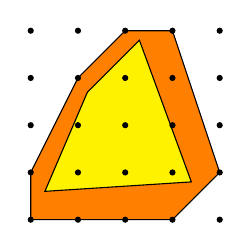
\begin{tikzpicture}[scale=0.6]
	\filldraw[fill=orange] (0,0) -- (0,1) -- (1,3) -- (2,4) -- (3,4) -- (4,1) -- (3,0) --cycle;
	\filldraw[fill=yellow] (0.3,0.6) -- (3.4,0.8) -- (2.3,3.8) --(1.2,2.7) -- cycle;
	\foreach \x in {0,...,4}
	\foreach \y in {0,...,4}
	{
		\filldraw[fill=black] (\x,\y)  circle (1.5pt);
	} 
	% \draw (1,0) -- (0,1) -- (2,2) --cycle;
	\end{tikzpicture}
\end{center}

Another option that is often favorable is \verb|DualMode| in connection with \verb|Deg1Elements|. So there are three choices for the computation of lattice points in polytopes:
\begin{itemize}
	\itemtt[Deg1Elements, -1] with local approximation of rational polytopes,
	\itemtt [Approximate Deg1Elements, -r1] combined with global approximation,
	\itemtt[DualMode Deg1Elements, -d1] dual mode optimized for the computation of degree $1$ elements.
\end{itemize}

Our demonstration example is \verb|max_polytope_cand| with the input file

\begin{Verbatim}
amb_space 5
inequalities 11
-3  -3 -10  14  88
26  -3  19  14 361
-4  25   6 -49 133
2  -3   1   5  17
-2  -3  -7  11  61
-6  23   9 -30 233
-2   7   3  -9  81
-8  17  12 -65 183
8 -15   4  23  65
-8 -13 -28  45 241
-8  27  12 -35 321  
grading
unit_vector 5
Approximate
Deg1Elements
\end{Verbatim}
set up for global approximation. (This is not a random input file; it has come up in connection with the paper ``Quantum jumps of normal polytopes'' by  W. Bruns, J. Gubeladze and M. Micha\l{}ek, arXiv:1504.01036.)

Despite of the large number of lattice points, the computation is extremely fast. Now remove \verb|Approximate|. This will take considerably longer, but will not overstretch your patience. Note that Normaliz will pass to GMP integers, which becomes necessary because of the huge determinants of the simplicial cones (without approximation).

The third choice using the dual algorithm is still o.k. though it takes the most time in this case. In other cases it may very well be the fastest.

You can also use inhomogeneous input with the default computation mode or dual mode. This is equivalent to homogeneous input with \verb|Deg1Elements| and \verb|DualMode|, respectively, in addition.

\subsection{The bottom decomposition}\label{bottom_dec}

The triangulation size and the determinant sum of the triangulation are critical size parameters in Normaliz computations. Normaliz always tries to order the generators in such a way that the determinant sum is close to the minimum, and on the whole this works out well. The use of the bottom decomposition by \verb|BottomDecomposition, -b| enables Normaliz to compute a triangulation with the optimal determinant sum for the given set of generators, as we will explain in the following. 

The determinant sum is independent of the order of the generators of the cone $C$ if they lie in a hyperplane $H$. Then the determinant sum is exactly the normalized volume of the polytope spanned by $0$ and $C\cap H$. The triangulation itself depends on the order, but the determinant sum is constant.
\begin{center}
	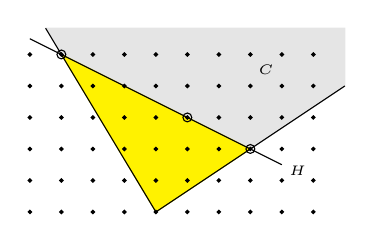
\begin{tikzpicture}[scale=0.4]
	\filldraw[gray!20] (-3.5,5.833) -- (0,0) -- (6,4) -- (6,5.833) -- cycle;
	\filldraw[yellow] (0,0) -- (-3,5) -- (3,2) -- cycle;
	\draw (-3.5,5.833) -- (0,0) -- (6,4);
	\foreach \x in {-4,...,5}
	\foreach \y in {0,...,5}
	{
		\filldraw[fill=black] (\x,\y)  circle (1.5pt);
	}
	\draw (-4,5.5) --(4,1.5) node at (4.5,1.3){\tiny $H$};
	
	\draw (-3,5) circle (4pt) node at (3.5,4.5){\tiny $C$};
	\draw (1,3) circle (4pt);
	\draw (3,2) circle (4pt); 
	\end{tikzpicture}
\end{center}

This observation helps to find a triangulation with minimal determinant sum in the general case.
We look at the \emph{bottom} (the union of the compact faces) of the polyhedron generated by $x_1,\dots,x_n$ as vertices and $C$ as recession cone, and take the volume underneath the bottom: 
\begin{center}
	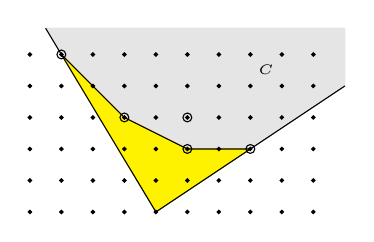
\begin{tikzpicture}[scale=0.4]
	\filldraw[gray!20] (-3.5,5.833) -- (0,0) -- (6,4) -- (6,5.833) -- cycle;
	\filldraw[yellow] (0,0) -- (-3,5) -- (-1,3) -- (1,2) -- (3,2) -- cycle;
	
	\draw (-3,5) -- (-1,3) -- (1,2) -- (3,2);
	
	\draw (-3.5,5.833) -- (0,0) -- (6,4);
	\foreach \x in {-4,...,5}
	\foreach \y in {0,...,5}
	{
		\filldraw[fill=black] (\x,\y)  circle (1.5pt);
	}
	
	\draw (-3,5) circle (4pt) node at (3.5,4.5){\tiny $C$};
	\draw (-1,3) circle (4pt);
	\draw (1,3) circle (4pt);
	\draw (3,2) circle (4pt);
	\draw (1,2) circle (4pt);  
	\end{tikzpicture}
\end{center}
With the option \texttt{BottomDecomposition}, \texttt{-b}, Normaliz 3.0 computes a triangulation that respects the bottom facets. This yields the optimal determinant sum for the given generators. If one can compute the Hilbert basis by the dual algorithm, it can be used as input, and then one obtains the absolute bottom of the cone, namely the compact facets of the convex hull of all nonzero lattice points. 

Normaliz does not always use the bottom decomposition by default since its computation requires some time and administrative overhead. However, as soon as the input ``profile'' is considered to be ``rough'' it is invoked. The measure of roughness is the ratio between the maximum degree (or $L_1$ norm without a grading) and the minimum. A ratio $\ge 5$ activates the bottom decomposition.

The bottom decomposition is part of the subdivision of large simplicial cones discussed in the next section.

Also see Section \ref{ele3}.

Note: the bottom decomposition cannot be activated by Normaliz if \verb|KeepOrder| is used. In this case \verb|BottomDecomposition| must be set explicitly if it is wanted.


\subsection{Subdivision of large simplicial cones}

Especially in computations with rational polytopes one encounters very large determinants that can keep the Normaliz primal algorithm from terminating in reasonable time. As an example we take \verb|hickerson-18.in| from the LattE distribution \cite{LatInt}. It is simplicial and the complexity is totally determined by the large determinant $\approx 4.17\times 10^{14}$ (computed with \verb|-v|). 

If we are just interested in the degree $1$ points, Normaliz uses the approximation method of Section \ref{approx} and finds $44$ degree $1$ points very quickly. If we use these points together with the extreme rays of the simplex, then the determinant sum decreases to $\approx 1.3\times 10^{12}$, and the computation of the Hilbert basis and the Hilbert series is in reach. But it is better to pursue the idea of subdividing large simplicial cones systematically. Normaliz employs two methods:
\begin{arab}
\item computation of subdivision points by the IP solver SCIP,
\item computation of candidate subdivision points by approximation of the given simplicial cone by an overcone that is generated by vectors  of `low denominator''.
\end{arab}

Normaliz tries to subdivide a simplicial cone if it has determinant $\ge 10^8$. Both methods are used recursively via stellar subdivision until simplicial cones with determinant $< 10^6$ have been reached or no further improvement is possible. All subdivision points are then collected, and the start simplicial cone is subdivided with bottom decomposition, which in general leads to substantial further improvement.

The use of SCIP requires a Normaliz executable that is compiled with the option \verb|SCIP=yes| after the installation of SCIP. Without SCIP only the approximation method is used. However, it can happen that SCIP fails because the required precision cannot be reached by floating point calculations. In this vase the approximation method will be tried as well. 

The following table contains some performance data for subdivisions based on SCIP (parallelization with 20 threads).
\begin{center}
\setlength{\tabcolsep}{3.2pt}
\renewcommand{\arraystretch}{1.2}
\begin{tabular}{|c|c|c|c|}
\hline
& \ttt{hickerson-16} & \ttt{hickerson-18} & \ttt{knapsack\_11\_60}  \\ \hline
simplex volume & $9.83\times 10^7$ & $4.17\times 10^{14}$ & $2.8\times 10^{14}$ \\ \hline
volume under bottom  & $8.10\times 10^5$ & $3.86\times 10^7$ & $2.02\times 10^7$ \\ \hline 
volume used     & $3.93\times 10^6$ & $5.47\times 10^7$ & $2.39\times 10^7$ \\ \hline
%improvement factor & 25 &  $7.62\times10^6$ & $1.17\times 10^7$\\ \hline
runtime without subdivision   &  2 s & >12 d &  >8 d \\ \hline
runtime with subdivision    &  0.5 s & 46 s & 5.1 s \\ \hline
\end{tabular}
\end{center}

Performance data for approximation:

\begin{center}
\setlength{\tabcolsep}{3.2pt}
\renewcommand{\arraystretch}{1.2}
\begin{tabular}{|c|c|c|c|}
\hline
& \ttt{hickerson-16} & \ttt{hickerson-18} & \ttt{knapsack\_11\_60}  \\ \hline
volume used     & $3.9 \times 10^6$ & $9.1\times 10^7$ & $2.3\times 10^9$ \\ \hline
%improvement factor & 25 &  $7.62\times10^6$ & $9.4\times 10^9$\\ \hline
runtime with subdivision    & 0.7 s & 58 s& 2 m 36 s\\ \hline
\end{tabular}
\end{center}

A good nonsimplicial example showing the subdivision at work is \verb|hickerson_18plus1.in|.

Note: After subdivision the decomposition of the cone may no longer be a triangulation in the strict sense, but a decomposition that we call a \emph{nested triangulation}; see \ref{nested}.

\subsection{Primal vs. dual -- division of labor}

The choice between the primal and the dual algorithm for Hilbert basis computations is presently left to the user. Normaliz does not make a guess which algorithm might be faster. If the number of support hyperplanes is small relative to the dimension, then the dual algorithm can be much faster. This is in particular true for (in)homogeneous linear systems of equations where the number of support hyperplanes is bounded above by the number of indeterminates ($+1$ in the inhomogeneous case).
The paper \cite{BIS} contains computation times for many examples that can help the user to choose the right algorithm. Note that the dual algorithm is arithmetically less critical than the primal algorithm since it basically only requires addition of vectors.

When both Hilbert basis and Hilbert series are to be computed, the best solution can be the combination of both algorithms. We recommend \verb|2equations.in| as a demonstration example which combines the algorithmic variant \verb|DualMode| abd the computation goal \verb|HilbertSeries|:
\begin{Verbatim}
amb_space 9
equations 2
1 6 -7 -18 25 -36 6 8 -9
7 -13 15 6 -9 -8 11 12 -2
total_degree
DualMode
HilbertSeries
\end{Verbatim}
The computation time (20 parallel threads) is 2 m 54 s whereas the default mode needs ???.

In addition to showing that the combination of the primal and dual algorithm can be very useful, it also shows the power of the the subdivision of large simplicial cones and bottom decomposition: while the ``raw'' determinant sum is $\approx 7.7\times 10^{11}$ (you can compute it with the options \verb|-iv|), the determinant sum of the Hilbert series computation is only $\approx 8.4\times 10^9$.

\subsection{Explicit dehomogenization}\label{dehom_ex}
Inhomogeneous input for data in $\RR^{d}$ is homogenized by an extra $(d+1)$th coordinate, The dehomogenization sets the last coordinate equal to $1$. Other systems may prefer the first coordinate. By choosing an explicit dehomogenization Normaliz can be adapted to such input. The file \verb|dehomogenization.in|
\begin{Verbatim}
amb_space 3
inequalities 2
-1 1 0
-1 0 1
dehomogenization
unit_vector 1
\end{Verbatim}
indicates that in this case the first variable is the homogenizing one. The output file
\begin{Verbatim}
1 module generators
2 Hilbert basis elements of recession monoid
1 vertices of polyhedron
2 extreme rays of recession cone
2 support hyperplanes of polyhedron

embedding dimension = 3
affine dimension of the polyhedron = 2 (maximal)
rank of recession monoid = 2

size of triangulation   = 0
resulting sum of |det|s = 0

dehomogenization:
1 0 0 


module rank = 1

***********************************************************************

1 module generators:
1 1 1

2 Hilbert basis elements of recession monoid:
0 0 1
0 1 0

1 vertices of polyhedron:                   2 support hyperplanes of polyhedron:
1 1 1                                       -1 0 1
                                            -1 1 0
2 extreme rays of recession cone:
0 0 1
0 1 0
\end{Verbatim}
shows that Normaliz does the computation in the same way as with implicit dehomogenization, except that now the first coordinate decides what is in the polyhedron and what belongs to the recession cone, roughly speaking.

Note that the dehomogenization need not be a coordinate. It can be any linear form that is nonnegative on the cone generators.

\subsection{Exporting the triangulation}

The option \ttt{-T} asks Normaliz to export the triangulation by writing the files 
writes \ttt{<project>.tgn} and \verb|<project>.tri|:

\begin{itemize}
	
	\itemtt[tgn]     The file \ttt{tgn} contains a matrix of vectors (in the
	coordinates of $\AA$) spanning the simplicial cones in
	the triangulation.
	
	\itemtt[tri]
	The file \ttt{tri} lists the simplicial subcones as follows:
	The first line contains the number of simplicial cones
	in the triangulation, and the next line contains the
	number $m+1$ where $m=\rank \EE$. Each of the following
	lines specifies a simplicial cone $\Delta$: the first
	$m$ numbers are the indices (with respect to the order
	in the file \ttt{tgn}) of those generators that span
	$\Delta$, and the last entry is the multiplicity of
	$\Delta$ in $\EE$, i.~e.\ the absolute value of the
	determinant of the matrix of the spanning vectors (as
	elements of $\EE$).
\end{itemize}

The following example is the $2$-dimensional cross polytope with one excluded face (\verb|cross2.in|). The excluded face is irrelevant for the triangulation.

\begin{Verbatim}
amb_space 3
polytope 4                           
1  0                      
0  1                
-1  0
0 -1
excluded_faces 1
1  1 -1                         
\end{Verbatim}

Its \verb|tgn| and \verb|tri| files are
\begin{Verbatim}
tgn             tri
4               2
3               4
1 0 1           1 2 3 2
0 1 1           1 3 4 2
-1 0 1          plain
0 -1 1                 
\end{Verbatim}

We see the $4$ vertices $v_1,\dots,v_4$ in homogenized coordinates in \verb|tgn| and the $2$ simplices (or the simplicial cones over them) in \verb|tri|: both have multiplicity $2$. The last word \verb|plain| indicates that Normaliz has computed a triangulation in the strict sense, namely a simplicial subdivision in which neighboring simplicial cones match along common faces. The alternative is \verb|nested| that we discuss below.

In addition to the files \verb|<project>.tgn| and \verb|<project>.tri|, also the file \verb|<object>.inv| is written. It contains the data of the file \verb|<project>.out| above the line of stars in a human and machine readable format.

\subsubsection{Nested triangulations}\label{nested}

If Normaliz has subdivided a simplicial cone of a triangulation of the cone $C$, the resulting decomposition of $C$ may no longer be a triangulation in the strict sense. It is rather a \emph{nested triangulation}, namely a map from a rooted tree to the set of full-dimensional subcones of $C$ with the following properties:
\begin{arab}
\item the root is mapped to $C$,
\item every other node is mapped to a full dimensional simplicial subcone,
\item the simplicial subcones corresponding to the branches at a node $x$ form a triangulation of the simplicial cone corresponding to $x$.
\end{arab}

The following figure shows a nested triangulation:

\begin{center}
	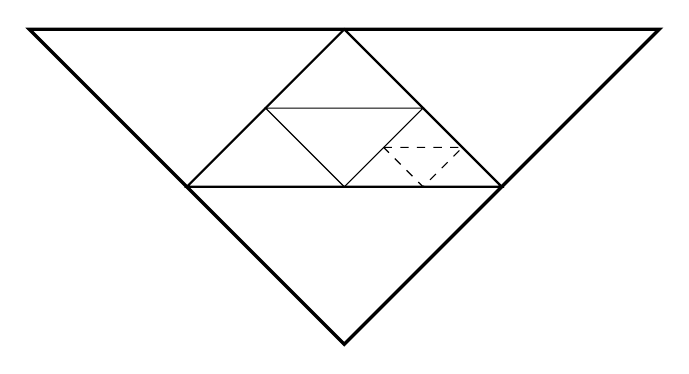
\begin{tikzpicture}[scale=1.0]
	\draw[very thick] (-4,4)  -- (4,4) -- (0,0) -- cycle;
	\draw[thick] (-2,2) -- (2,2) -- (0,4) -- cycle;
	\draw (-1,3) -- (1,3) -- (0,2) -- cycle;
	\draw[dashed] (0.5,2.5) --(1.5,2.5) -- (1.0,2) --cycle;
\end{tikzpicture}
\end{center}

For the Normaliz computations, nested triangulations are as good as ordinary triangulations, but in other applications the difference may matter. With the option \verb|-T|, Normaliz prints the leaves of the nested triangulation to the \verb|tri| file. They constitute the simplicial cones that are finally evaluated by Normaliz.

The triangulation is always plain if \verb|-T| is the only computation goal or if it is just combined with \verb|-v|. Otherwise it can only fail to be plain if it contains determinants $\ge 10^8$.


\subsection{Exporting the Stanley decomposition}

The option \ttt{-y} makes Normaliz 
write the files  \ttt{<project>.tgn}, \verb|<project>.dec| and \verb|<project>.inv|.   Stanley decomposition is contained in the file with the suffix \verb|dec|. But this file also contains the inclusion/exclusion data if there are excluded faces:

(a) If there are any excluded faces, the file starts with the word
\verb|in_ex_data|. The next line contains the number of such data that follow.
Each of these lines contains the data of a face and the coefficient with which
the face is to be counted: the first number lists the number of generators that
are contained in the face, followed by the indices of the generators relative
to the \verb|tgn| file and the last number is the coefficient.

(b) The second block (the first if there are no excluded faces) starts with
the word \verb|Stanley_dec|, followed by the number of simplicial cones in the
triangulation.

For each simplicial cone $\Delta$ in the
triangulation this file contains a block of data:
\begin{enumerate}
	\item[(i)] a line listing the indices $i_1,\dots,i_m$ of the
	generators $v_{i_1},\dots,v_{i_m}$ relative to the
	order in \ttt{tgn} (as in \ttt{tri}, $m=\rank \EE$);
	
	\item[(ii)] a $\mu\times m$ matrix where $\mu$ the
	multiplicity of $\Delta$ (see above).
	
	In the notation of \cite{BIS}, each line lists an
	``offset'' $x+\epsilon(x)$  by its coordinates with
	respect to $v_{i_1},\dots,v_{i_m}$ as follows: if
	$(a_1,\dots,a_m)$ is the line of the matrix, then
	$$
	x+\epsilon(x)=\frac{1}{\mu}(a_1v_{i_1}+\dots+a_mv_{i_m}).
	$$
\end{enumerate}


The \verb|dec| file of the example above is
\begin{Verbatim}
in_ex_data
1
2 1 2 -1
Stanley_dec
2
1 3 4              1 2 3 
2                  2     
3                  3     
0 0 2              0 0 0 
1 1 2              1 0 1
\end{Verbatim}

There is $1$ face in \verb|in_ex_data| (namely the excluded one), it contains the $2$ generators $v_1$ and $v_2$  and appears with multiplicity $-1$. The Stanley decomposition consists of $4$ components of which each of the simplicial cone contains $2$. The second offset in the second simplicial cone is
$$
\frac12 (1v_1+0v_2+1v_3)=(0,0,1).
$$ 

The file \ttt{3x3magiceven.in} has been processed with the
option \ttt{-ahTy} activated. We recommend you to inspect all
the output files in the subdirectory \ttt{example} of the
distribution.

\subsection{Minimal module generators of the integral closure}\label{MinMod}

Suppose that the original generators are well defined in the input. This is always the case when these consists just of a \verb|cone| or a \verb|cone_and_lattice|. Let $M$ be the monoid generated by them. Then Normaliz computes the integral closure $N$ of $M$ in the effective lattice $\EE$. It is often interesting to understand the difference set $N\setminus M$. After the introduction of a field $K$ of coefficients, this amounts to understanding the quotient $K[N]/K[M]$ as a $K[M]$-module. With the option \verb|ModuleGeneratorsofIntegralClosure, -M| Normaliz computes a minimal generating set $T$ of this module. Combinatorially this means that we find an irreducible  cover
$$
N\setminus M\subset\bigcup_{x\in T} x+M.
$$
\begin{center}
	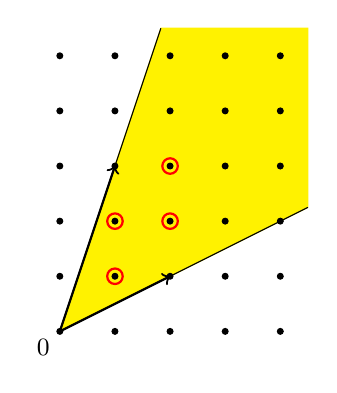
\begin{tikzpicture}[scale=0.7]
	\filldraw[yellow] (0,0) -- (1.833,5.5) -- (4.5,5.5) -- (4.5,2.25) -- cycle;
	\draw (0,0) -- (1.833,5.5);
	\draw (0,0) -- (4.5,2.25) node at (-0.3,-0.3){\small $0$};
	\foreach \x in {0,...,4}
	\foreach \y in {0,...,5}
	{
		\filldraw[fill=black] (\x,\y)  circle (1.5pt);
	}
	\draw[red,thick] (1,1) circle (4pt);
	\draw[red,thick] (2,3) circle (4pt);
	\draw[red,thick] (1,2) circle (4pt);
	\draw[red,thick] (2,2) circle (4pt);
	\draw[->,thick] (0,0) -- (1,3);
	\draw[->,thick] (0,0) -- (2,1);
	\end{tikzpicture}
\end{center}
As an example, we can run \verb|2cone.in| with the option \verb|-M| on the command line. This yields the output
\begin{Verbatim}
...
4 Hilbert basis elements:
1 1
1 2
1 3
2 1

2 extreme rays:          4 module generators of integral closure/original monoid:
1 3                      1 1
2 1                      1 2
                         2 2
                         2 3
\end{Verbatim} 


\subsection{Precomputed support hyperplanes}\label{supphyp_ex}

Computing the support hyperplanes can be a very time consuming task, and if it has been the first step in the exploration of a difficult example, it may be desirable, to use the support hyperplanes as additional input in order to save computation time. This is especially true if Normaliz must do an intermediate computation of the support hyperplanes because of a large number of simplicial cones to be evaluated. The file \verb|2cone_supp.in| is just a toy example:
\begin{Verbatim}
amb_space 2
cone 2
2 1
1 3
inequalities 2
-1  2
 3 -1
\end{Verbatim}

As pointed out in Section \ref{HomConstrCone}, Normaliz must trust you---here is no way of checking the correctness of this input without recomputing it.

\subsection{A very large computation}\label{ele3}

The example \verb|CondEffPlur.in| is one of the largest that Normaliz has mastered. The goal is to compute the Condorcet efficiency of plurality voting for $4$ candidates  (see \cite{BS} and the references therein), even in the refined form of the Hilbert series. The Hilbert basis computation is extremely fast in \verb|DualMode| so that it can be used as input. We tried three different setups (each with $30$ parallel threads): 

\begin{center}
	\begin{tabular}{|r|r|r|r|}\hline
		input	& triangulation size& determinant sum& computation time\\ \hline
		inequalities & 347,225,775,338 &4,111,428,313,448  & 112:43:17 h\\ \hline
		inequalities \ttt{-b} & 288,509,390,884 & 1,509,605,641,358 & 84:26:19 h\\ \hline
		Hilbert basis, \ttt{-b}& 335,331,680,623&1,433,431,230,802& 97:50:05 h \\ \hline
	\end{tabular}
\end{center}

The results show that the determinant sum of the bottom decomposition based on th extreme rays (resulting from dualizing the input cone) comes very close to the absolute minimum that is reached by the Hilbert basis as input. The latter leads to a finer triangulation, which, despite of the smaller determinant sum, increases the computation time.

As long as the determinants are rather small (as in this computation), the two cases $\det=1$ and $\det>1$ make the difference in computation complexity. In the first case Normaliz must solve $1$ or $2$ linear systems for the simplicial cone, in the latter $2$ or $3$. 

Note: though Normaliz can compute this example, it is really a case for NmzIntegrate; see \cite{BIS}. It converts the computation time from days to hours.


\section{Optional output files}\label{optionaloutput}


When one of the options \ttt{Files,-f} or \ttt{AllFiles, -a}, Normaliz
writes additional output files whose names are of type
\ttt{<project>.<type>}. (Note that the options \verb|-T, Triangulation| and \verb|-y, StanleyDec| as well as the options calling NmzIntegrate also write files in addition to \verb|<project>.out|.) Moreover one can select the optional output files individually via command line options. Most of these files contain matrices in a simple format:
\begin{Verbatim}
<m>
<n>
<x_1>
...
<x_m>
\end{Verbatim}
where each row has \verb|<n>| entries. Exceptions are the files with suffixes \verb|cst|, \verb|inv|, \verb|esp|.

\subsection{The homogeneous case}

The option \ttt{-f} makes Normaliz write the following files:

\begin{itemize}
	\itemtt[gen] contains the Hilbert basis.
	
	\itemtt[cst] contains the constraints defining the cone
	and the lattice in the same format as they would appear
	in the input: matrices of types \emph{constraints} following each
	other. Each matrix is concluded by the type of the constraints.
	Empty matrices are indicated by $0$ as the
	number of rows. Therefore there will always be at least
	$3$ matrices.
	
	If a grading is defined, it will be appended. Therefore
	this file (with suffix \ttt{in}) as input for
	Normaliz will reproduce the Hilbert basis and all the
	other data computed, at least in principle.
	
	\itemtt[inv]  contains all the information from the
	file \ttt{out} that is not contained in any of the
	other files.
\end{itemize}

If \ttt{-a} is activated, then the following files are written
\emph{additionally:}

\begin{itemize}
	
	\itemtt[ext] contains the extreme rays of the cone.
	
	\itemtt[ht1] contains the degree $1$ elements of the
	Hilbert basis if a grading is defined.
	
	\itemtt[egn,esp] These contain the Hilbert basis and
	support hyperplanes in the coordinates with respect to
	a basis of $\EE$. \ttt{esp} contains the grading and the dehomogenization in the
	coordinates of $\EE$. Note that no
	equations for $\CC\cap\EE$ or congruences for $\EE$ are
	necessary.
	
    \itemtt[lat] contains the basis of the lattice $\EE$.

    \itemtt[mod] contains the module generators of the integral closure modulo the original monoid.
\end{itemize}

In order to select one or more of these files individually, add an option of type \verb|--<suffix>| to the command line where \verb|<suffix>| can take the values
\begin{Verbatim}
gen, cst, inv, ext, ht1, egn, esp, lat, mod, typ
\end{Verbatim}

The type \verb|typ| is not contained in \verb|Files| or \verb|AllFiles| since it can be extremely large. It is the matrix format described above. It is the product of the matrices
corresponding to \ttt{egn} and the transpose of \ttt{esp}. In other
words, the linear forms representing the support
hyperplanes of the cone $C$ are evaluated on the
Hilbert basis. The resulting matrix, with the
generators corresponding to the rows and the support
hyperplanes corresponding to the columns, is written to
this file.

The suffix \ttt{typ} is motivated by the fact that the
matrix in this file depends only on the isomorphism
type of monoid generated by the Hilbert basis (up to
row and column permutations). In the language of
\cite{BG} it contains the \emph{standard embedding}. 

Note: the explicit choice of an optional output file does \emph{not} imply a computation goal. Output files that would contain unknown data are simply not written without a warning or error message.

\subsection{Modifications in the inhomogeneous case}

The optional output files  are a subset of those that can be produced in the homogeneous
case. The main difference is that the generators of the solution module and the
Hilbert basis of the recession monoid appear together in the file \verb|gen|.
They can be distinguished by evaluating the dehomogenization on them (simply the last component with inhomogeneous input), and the
same applies to the  vertices of the polyhedron and extreme rays of the
recession cone. The file \verb|cst| contains the constraints defining the
polyhedron and the recession module in conjunction with the dehomogenization, which is also contained in the \verb|cst| file, following the constraints.

With \verb|-a| the files \verb|egn| and \verb|esp| are produced. These files contain \verb|gen| and the support hyperplanes of the homogenized cone in the coordinates of $\EE$, as well as the dehomogenization.

%%%%%%%%%%%%%%%%%%%%%%%%%%%%  TERMINAL OUTPUT  %%%%%%%%%%%%%%%%%%%%%%%%%%%%%

%\section{Terminal output}

%%%%%%%%%%%%%%%%%%%%%%%%%%%%  PERFORMANCE AND PARALLELIZATION  %%%%%%%%%%%%%%%%%%%%%%%%%%%%%



%%%%%%%%%%%%%%%%%%%%%%%%%%%%%  LARGE COMPUTATIONS  %%%%%%%%%%%%%%%%%%%%%%%%%%%%%

\section{Performance}\label{Perf}

\subsection{Parallelization}\label{PerfPar}

The executables of Normaliz have been compiled for parallelization
on shared memory systems with OpenMP. Parallelization reduces the
``real'' time of the computations considerably, even on relatively
small systems. However, one should not underestimate the
administrational overhead involved.
\begin{itemize}
	\item It is not a good idea to use parallelization for very small problems.
	\item On multi-user systems with many processors it may be wise to limit
	the number of threads for Normaliz somewhat below the maximum
	number of cores.
\end{itemize}
The number of parallel threads can be limited by the Normaliz
option \ttt{-x} (see Section \ref{exec}) or by the commands
\begin{center}
	\verb+export OMP_NUM_THREADS=<T>+\qquad (Linux/Mac)
\end{center}
or
\begin{center}
	\verb+set OMP_NUM_THREADS=<T>+\qquad (Windows)
\end{center}
where \ttt{<T>} stands for the maximum number of threads
accessible to Normaliz. For example, we often use
\begin{center}
	\verb+export OMP_NUM_THREADS=20+
\end{center}
on a multi-user system system with $24$ cores.

Limiting the number of threads to $1$ forces a strictly serial
execution of Normaliz.

The paper \cite{BIS} contains extensive data on the effect of parallelization. On the whole Normaliz scales very well.
However, the dual algorithm often performs best with mild parallelization, say with $4$ or $6$ threads.

\subsection{Running large computations}\label{Large}

Normaliz can cope with very large examples, but  it
is usually difficult to decide a priori whether an example is
very large, but nevertheless doable, or simply impossible.
Therefore some exploration makes sense.

See \cite{BIS} for some very large computations. The following
hints reflect the authors' experience with them.

(1) Run Normaliz with the option \ttt{-cs} and pay attention
to the terminal output. The number of extreme rays, but also
the numbers of support hyperplanes of the intermediate cones
are useful data.

(2) In many cases the most critical size parameter is the
number of simplicial cones in the triangulation. It makes sense
to determine it as the next step. Even with the fastest
potential evaluation (option \ttt{-v}), finding the
triangulation takes less time, say by a factor between $3$ and
$10$. Thus it makes sense to run the example with \ttt{-t} in
order to explore the size.

As you can see from \cite{BIS}, Normaliz has successfully
evaluated triangulations of size $\approx 5\cdot 10^{11}$ in
dimension $24$.

(3) Another critical parameter are the determinants of the
generator matrices of the simplicial cones. To get some feeling
for their sizes, one can restrict the input to a subset (of the
extreme rays computed in (1)) and use the option \ttt{-v} or the computation goal \verb|DeeterminantSum| if there is no grading.

The output file contains the number of simplicial cones as well
as the sum of the absolute values of the determinants. The
latter is the number of vectors to be processed by Normaliz
in triangulation based calculations.

The number includes the zero vector for every simplicial cone
in the triangulation. The zero vector does not enter the
Hilbert basis calculation, but cannot be neglected for the
Hilbert series.

Normaliz has mastered calculations with $> 10^{15}$ vectors.

(4) If the triangulation is small, we can add the option
\ttt{-T} in order to actually see the triangulation in a file.
Then the individual determinants become visible.

(5) If a cone is defined by inequalities and/or equations
consider the dual mode for Hilbert basis calculation, even if
you also want the Hilbert series.

(6) The size of the triangulation and the size of the
determinants are \emph{not} dangerous for memory by themselves
(unless \ttt{-T} or \ttt{-y} are set). Critical magnitudes can
be the number of support hyperplanes, Hilbert basis candidates,
or degree $1$ elements.

%%%%%%%%%%%%%%%%%%%%%%%%%%%%%  DISTRIBUTION  %%%%%%%%%%%%%%%%%%%%%%%%%%%%%
\section{Distribution and installation}\label{Distr}

In order to install Normaliz you should first download the
basic package containing the documentation, examples, source
code, jNormaliz, NmzIntegrate and the packages for Singular
and Macaulay2. Then unzip the downloaded file
\ttt{Normaliz3.0.zip} in a directory of your choice. (Any other
downloaded zip file for Normaliz should be unzipped in this
directory, too.)

This process will create a directory \ttt{Normaliz3.0} (called
Normaliz directory) and several subdirectories in
\ttt{Normaliz3.0}. The names of the subdirectories created are
self-explanatory. Nevertheless we give an overview:
\begin{itemize}
	\item In the main directory \ttt{Normaliz3.0} you should
	find \ttt{jNormaliz.jar}, \ttt{Copying} and
	subdirectories.
	
	\item The subdirectory \ttt{source} contains the source
	files and a \ttt{Makefile} for compilation with GCC.
	The subdirectory \ttt{genEhrhart} contains the
	NmzIntegrate source.
	
	\item The subdirectory \ttt{doc} contains the file you are
	reading and further documentation.
	
	\item In the subdirectory \ttt{example} are the input
	and output files for some examples. It contains all
	input files of examples of this documentation, except the toy
	examples of Section \ref{input}. Some very large output files
	are contained in an extra zip file accessible from the
	Normaliz home page.
	
	\item The subdirectory \ttt{singular} contains the
	\textsc{Singular} library \ttt{normaliz.lib} and a PDF file with
	documentation.
	
	\item The subdirectory \ttt{macaulay2} contains the
	\textsc{Macaulay2} package \ttt{Normaliz.m2}.
	\item The subdirectory \ttt{lib} contains libraries for
	jNormaliz.
\end{itemize}

We provide executables for Windows, Linux (each in a 32 bit and
a 64 bit version) and Mac. Download the archive file
corresponding to your system \ttt{Normaliz3.0<systemname>.zip}
and unzip it. This process will store the executables of
Normaliz and NmzIntegrate in the directory
\ttt{Normaliz3.0}. In case you want to run Normaliz from the
command line or use it from other systems, you may have to copy
the executables to a directory in the search path for
executables.

Please remove old versions of \ttt{normaliz}, \ttt{norm64} and \ttt{normbig}
from your search path.

Running NmzIntegrate requires the additional download of its
executable for your system.


%%%%%%%%%%%%%%%%%%%%%%%%%%%%%  COMPILATION  %%%%%%%%%%%%%%%%%%%%%%%%%%%%%
\section{Compilation}\label{Compile}

We only describe the compilation of Normaliz. See the
documentation of NmzIntegrate for its compilation.

\subsection{GCC}


Produce the executables by calling \ttt{make} in the subdirectory
\ttt{source}. You may have to transport the executables to a
directory in your search path. \textbf{jNormaliz expects them in
	its own directory.}

Note that \ttt{normaliz} needs GMP (including the C++ wrapper) and
the Boost collection. Therefore you must install them first.

We are using OpenMP 3.0. Please make sure that your GCC version is
compatible with it (version $\ge$ 4.4).

Note the following \textbf{exceptions:}
\begin{enumerate}
	\item One can compile Windows executables with the Cygwin
	port of GCC. Unfortunately it is not compatible to
	OpenMP.
	\item Mac versions of GCC older than 4.5 have a bug that
	makes it impossible to use OpenMP.
\end{enumerate}
In any case, or if you want to avoid parallelization, you can
call \texttt{make OPENMP=no}.

\subsection{Visual Studio project}

The Windows executables provided by us have been compiled with
MS Visual Studio and Intel C++ Composer XE. (Visual C++ itself can
only be used without OpenMP.)

If you want to compile Normaliz yourself in this way, please unzip
the corresponding zip file on the Normaliz home page. This will
create a subdirectory \ttt{Visual Studio} of the Normaliz
directory. This directory contains the predefined project. We have
provided

\begin{enumerate}
	\item two configurations: \ttt{Release} (with OpenMP) and
	\ttt{ReleaseSerial} (without OpenMP), and
	\item two platforms, \ttt{Win32} and \ttt{x64}.
\end{enumerate}

Instead of GMP we use the MPIR library for the Windows version
of \ttt{normaliz}. For convenience, the MPIR files have been
included in the distribution (in the subdirectory \ttt{MPIR} of
\ttt{Visual Studio}). Please
\begin{itemize}
	\item copy the library files for Win32 into the \ttt{lib}
	subdirectory of the Visual C++ compiler,
	
	\item the library files for x64 to the subdirectory
	\ttt{amd64} (or \ttt{x64}) of \ttt{lib}, and
	
	\item the two header files to the \ttt{include}
	subdirectory of the compiler.
\end{itemize}
Moreover, you must install the Boost collection available from
http://www.boost.org/. We only use Boost libraries that are
entirely implemented in their headers. So the only preparation
beyond downloading and unzipping is to add the Boost root
directory to the list of include paths. In the Visual Studio C++ IDE,
click ``Tools | Options... | Projects | VC++ directories''.
Then, in ``Show Directories for'', select ``Include files'' and
add the path to the Boost root directory.

After the compilation with the Intel compiler you must copy the executable
to the directories where they are expected (the Normaliz
directory or a directory in the search path).

The source files for Visual Studio are identical to those for GCC.



\section{Copyright and how to cite}

Normaliz 3.0 is free software licensed under the GNU General
Public License, version 3. You can redistribute it and/or
modify it under the terms of the GNU General Public License as
published by the Free Software Foundation, either version 3 of
the License, or (at your option) any later version.

It is distributed in the hope that it will be useful, but
WITHOUT ANY WARRANTY; without even the implied warranty of
MERCHANTABILITY or FITNESS FOR A PARTICULAR PURPOSE. See the
GNU General Public License for more details.

You should have received a copy of the GNU General Public
License along with the program. If not, see
http://www.gnu.org/licenses/.

Please refer to Normaliz in any publication for which it has
been used:
\begin{center}
	W. Bruns, B. Ichim, R. Sieg, T. R�mer and C. S�ger: Normaliz. Algorithms for
	rational cones and affine monoids. Available from
	http://www.math.uos.de/normaliz.
\end{center}
The corresponding \verb|\bibitem|:
\begin{Verbatim}
\bibitem W. Bruns, B. Ichim, R. Sieg, T. R�mer and C. S�ger: Normaliz. Algorithms
for rational cones and affine monoids. Available from
http://www.math.uos.de/normaliz.
\end{Verbatim}

It is now customary to evaluate mathematicians by such data as
numbers of publications, citations and impact factors. The data
bases on which such dubious evaluations are based do not list
mathematical software. Therefore we ask you to cite the article
\cite{BIS} in addition. This is very helpful for the younger
members of the team.

\newpage

\appendix

\section{Mathematical background and terminology}

For a coherent and thorough treatment of the mathematical background we refer the reader to \cite{BG}.

\subsection{Polyhedra, polytopes and cones}

An \emph{affine halfspace} of $\RR^d$ is a subset given as
$$
H_\lambda^+=\{x: \lambda(x)\ge 0\},
$$
where $\lambda$ is an affine form, i.e., a non-constant map $\lambda:\RR^d\to\RR$, $\lambda(x)=\alpha_1x_1+\dots+\alpha_dx_d+\beta$ with $\alpha_1,\dots,\alpha_d,\beta\in\RR$. If $\beta=0$ and $\lambda$ is therefore linear, then the halfspace is called \emph{linear}. The halfspace is \emph{rational} if $\lambda$ is \emph{rational},  i.e., has rational coordinates. If $\lambda$ is rational, we can assume that it is even \emph{integral}, i.e., has integral coordinates, and, moreover, that these are coprime. Then $\lambda$ is uniquely determined by $H_\lambda^+$. Such integral  forms are called \emph{primitive}, and the same terminology applies to vectors.

\begin{definition}
	A (rational) \emph{polyhedron} $P$ is the intersection of finitely many (rational) halfspaces. If it is bounded, then it is called a \emph{polytope}. If all the halfspaces are linear, then $P$ is a \emph{cone}.
	
	The \emph{dimension} of $P$ is the dimension of the smallest affine subspace $\aff(P)$ containing $P$.
\end{definition}


A support hyperplane of $P$ is an affine hyperplane $H$ that intersects $P$, but only in such a way that $H$ is contained in one of the two halfspaces determined by $H$. The intersection $H\cap P$ is called a \emph{face} of $P$. It is a polyhedron (polytope, cone) itself. Faces of dimension $0$ are called \emph{vertices}, those of dimension $1$ are called \emph{edges} (in the case of cones \emph{extreme rays}), and those of dimension $\dim(P)-1$ are \emph{facets}.

When we speak of \emph{the} support hyperplanes of $P$, then we mean those intersecting $P$ in a facet. Their halfspaces containing $P$ cut out $P$ from $\aff(P)$. If $\dim(P)=d$, then they are uniquely determined (up to a positive scalar).

The constraints by which Normaliz describes polyhedra are
\begin{arab}
	\item linear equations for $\aff(P)$ and
	\item linear inequalities (simply called support hyperplanes) cutting out $P$ from $\aff(P)$.
\end{arab}
In other words, the constraints are given by a linear system of equations and inequalities, and a polyhedron is nothing else than the solution set of a linear system of inequalities and equations. It can always be represented in the form
$$
Ax\ge b, \qquad A\in\RR^{m\times d}, b\in \RR^m,
$$
if we replace an equation by two inequalities.

\subsection{Cones}

The definition describes a cone by constraints. One can equivalently describe it by generators:

\begin{theorem}[Minkowski-Weyl]
	The following are equivalent for $C\subset\RR^d$;
	\begin{enumerate}
		\item $C$ is a (rational) cone;
		\item there exist finitely many (rational) vectors $x_1,\dots,x_n$ such that
		$$
		C=\{a_1x_1+\dots+a_nx_n:a_1,\dots,a_n\in\RR_+\}.
		$$
	\end{enumerate}
\end{theorem}

By $\RR_+$ we denote the set of nonnegative real numbers; $\QQ_+$ and $\ZZ_+$ are defined in the same way.

The conversion between the description by constraints and that by generators is one of the basic tasks of Normaliz. It uses the \emph{Fourier-Motzkin elimination}.

A cone is \emph{pointed} if $x\in C$ and $-x\in C$ is only possible with $x=0$. If a rational cone is pointed, then it has uniquely determined \emph{extreme integral generators}. These are the primitive integral vectors spanning the extreme rays. These can also be defined with respect to a sublattice $L$ of $\ZZ^d$, provided $C$ is contained in $\RR L$.

The \emph{dual cone} $C^*$ is given by
$$
C^*=\{\lambda\in (\RR^d)^*:\lambda(x)\ge0 \text{ for all } x\in C\}.
$$
Under the identification $\RR^d=(\RR^d)^{**}$ one has $C^{**}=C$. Let $C_0$ be the set of those $x\in C$ for which $-x\in C$ as well. It is the largest vector subspace contained in $C$. Then one has
$$
\dim C_0+\dim C^*=d.
$$
In particular, $C$ is pointed if and only if $C^*$ is full dimensional, and this is the criterion for pointedness used by Normaliz. Linear forms $\lambda_1,\dots,\lambda_n$ generate $C^*$ if and only if $C$ is the intersection of the halfspaces $H_{\lambda_i}^+$. Therefore the conversion from constraints to generators and its converse are the same task, except for the exchange of $\RR^d$ and its dual space.

\subsection{Polyhedra}

In order to transfer the Minkowski-Weyl theorem to polyhedra it is useful to homogenize coordinates by embedding $\RR^d$ as a hyperplane in $\RR^{d+1}$, namely via
$$
\kappa:\RR^d\to\RR^{d+1},\qquad \kappa(x)=(x,1).
$$
If $P$ is a (rational) polyhedron, then the closure of the union of the rays from $0$ through the points of $\kappa(P)$ is a (rational) cone $C(P)$, called the \emph{cone over} $P$. The intersection $C(P)\cap(\RR^d\times\{0\})$ can be identified with the \emph{recession} (or tail) \emph{cone}
$$
\rec(P)=\{x\in\RR^d: y+x\in P\text{ for all } y\in P\}.
$$
It is the cone of unbounded directions in $P$. The recession cone is pointed if and only if $P$ has at least one bounded face, and this is the case if and only if it has a vertex.

The theorem of Minkowski-Weyl can then be generalized as follows:

\begin{theorem}[Motzkin]
	The following are equivalent for a subset $P\neq\emptyset$  of $\RR^d$:
	\begin{enumerate}
		\item $P$ is a (rational) polyhedron;
		\item $P=Q+C$ where $Q$ is a (rational) polytope and $C$ is a (rational) cone.
	\end{enumerate}
	If $P$ has a vertex, then the smallest choice for $Q$ is the convex hull of its vertices, and $C=\rec(P)$ is uniquely determined.
\end{theorem}

The \emph{convex hull} of a subset $X\in\RR^d$ is
$$
\conv(X)=\{a_1x_1+\dots+a_nx_n: n\ge 1, x_1,\dots,x_n\in X, a_1,\dots,a_n\in\RR_+, a_1+\dots+a_n=1\}.
$$

Clearly, $P$ is a polytope if and only if $\rec(P)=\{0\}$, and the specialization to this case one obtains Minkowski's theorem: a subset $P$ of $\RR^d$ is a polytope if and only if it is the convex hull of a finite set. A \emph{lattice polytope} is distinguished by having integral points as vertices.

Normaliz computes the recession cone and the polytope $Q$ if $P$ is defined by constraints. Conversely it finds the constraints if the vertices of $Q$ and the generators of $C$ are specified.

Suppose that $P$ is given by a system
$$
Ax\ge b, \qquad A\in\RR^{m\times d},\ b\in \RR^m,
$$
of linear inequalities (equations are replaced by two inequalities). Then $C(P)$ is defined by the \emph{homogenized system}
$$
Ax-x_{d+1}b\ge 0
$$
whereas the $\rec(P)$ is given by the \emph{associated homogeneous system}
$$
Ax\ge 0.
$$

It is of course possible that $P$ is empty if it is given by constraints since inhomogeneous systems of linear equations and inequalities may be unsolvable. By abuse of language we call the solution set of the associated homogeneous system the recession cone of the system.

Via the concept of dehomogenization, Normaliz allows for a more general approach. The \emph{dehomogenization} is a linear form $\delta$ on $\RR^{d+1}$. For a cone $\widetilde C$ in $\RR^{d+1}$ and a dehomogenization $\delta$, Normaliz computes the polyhedron $P=\{x\in \widetilde C: \delta(x)=1\}$ and the recession cone $C=\{x\in \widetilde C: \delta(x)=0\}$. In particular, this allows other choices of the homogenizing coordinate. (Often one chooses $x_0$, the first coordinate then.)

In the language of projective geometry, $\delta(x)=0$ defines the hyperplane at infinity.

\subsection{Affine monoids}

An \emph{affine monoid} $M$ is a finitely generated submonoid of $\ZZ^d$ for some $d\ge0$. This means: $0\in M$, $M+M\subset M$, and there exist $x_1,\dots,x_n$ such that
$$
M=\{a_1x_1+\dots+a_nx_n: a_1,\dots,a_n\in\ZZ_+\}.
$$
We say that $x_1,\dots,x_n$ is a \emph{system of generators} of $M$. A monoid $M$ is positive if $x\in M$ and $-x\in M$ implies $x=0$.  An element $x$ in a positive monoid $M$ is called \emph{irreducible} if it has no decomposition $x=y+z$ with $y,z\in M$, $y,z\neq0$. The \emph{rank} of $M$ is the rank of the subgroup $\gp(M)$ of $\ZZ^d$ generated by $M$. (Subgroups of $\ZZ^d$ are also called sublattices.)
For certain aspects of monoid theory it is very useful (or even necessary) to introduce coefficients from a field $K$ (or a more general commutative ring) and consider the monoid algebra $K[M]$.


\begin{theorem}[van der Corput]
	Every positive affine monoid $M$ has a unique minimal system of generators, given by its irreducible elements.
\end{theorem}

We call the minimal system of generators the \emph{Hilbert basis} of $M$. Normaliz computes Hilbert bases of a special type of affine monoid:

\begin{theorem}[Gordan's lemma]
	Let $C\subset\RR^d$ be a (pointed) rational cone and let $L\subset \ZZ^d$ be a sublattice. Then $C\cap L$ is a (positive) affine monoid.
\end{theorem}

Let $M\subset \ZZ^d$ be an affine monoid, and let $N\supset M$ be an overmonoid (not necessarily affine), for example a sublattice $L$ of $\ZZ^d$ containing $M$.

\begin{definition}
	The \emph{integral closure} (or \emph{saturation}) of $M$ in $N$ is the set
	$$
	\widehat M_N=\{x\in N: kx\in M \text{ for some } k\in \ZZ, k>0\}.
	$$
	If $\widehat M_N=M$, one calls $M$ \emph{integrally closed} in $N$.
	
	The integral closure $\overline M$ of $M$ in $\gp(M)$ is its \emph{normalization}. $M$ is \emph{normal} if $\overline M=M$.
\end{definition}

The integral closure has a geometric description:

\begin{theorem}\label{incl_cone}
	$$
	\widehat M_N =\cone(M)\cap N.
	$$
\end{theorem}

Combining the theorems, we can say that Normaliz computes integral closures of affine monoids in lattices, and the integral closures are themselves affine monoids as well. (More generally, $\widehat M_N$ is affine if $M$ and $N$ are affine.)

In order to specify the intersection $C\cap L$ by constraints we need a system of homogeneous inequalities for $C$. Every sublattice of $\ZZ^d$ can be written as the solution set of a combined system of homogeneous linear diophantine equations and a homogeneous system of congruences (this follows from the elementary divisor theorem). Thus $C\cap L$ is the solution set of a homogeneous linear diophantine system of inequalities, equations and congruences. Conversely, the solution set of every such system is a monoid of type $C\cap L$.

In the situation of Theorem \ref{incl_cone}, if $\gp(N)$ has finite rank as a $\gp(M)$-module, $\widehat M_N$ is even a finitely generated module over $M$. I.e., there exist finitely many elements $y_1,\dots,y_m\in \widehat M_N$ such that $\widehat M_N=\bigcup_{i=1}^m M+y_i$. Normaliz computes a minimal system $y_1,\dots,y_m$ and lists the nonzero $y_i$ as a system of module generators of $\widehat M_N$ modulo $M$. We must introduce coefficients to make this precise: Normaliz computes a minimal system of generators of the $K[M]$-module $K[\widehat M_N]/K[M]$.

\subsection{Affine monoids from binomial ideals}\label{binomials}

Let $U$ be a subgroup of $\ZZ^n$. Then the natural image $M$ of
$\ZZ_+^n\subset\ZZ^n$ in the abelian group $G=\ZZ^n/U$ is a
submonoid of $G$. In general, $G$ is not torsionfree, and
therefore $M$ may not be an affine monoid. However, the image
$N$ of $M$ in the lattice $L=G/\textup{torsion}(G)$ is an affine
monoid. Given $U$, Normaliz chooses an embedding
$L\hookrightarrow\ZZ^r$, $r=n-\rank U$, such that $N$ becomes a
submonoid of $\ZZ_+^r$. In general there is no canonical choice
for such an embedding, but one can always find one, provided
$N$ has no invertible element except $0$. 

The typical starting point is an ideal $J\subset
K[X_1,\dots,X_n]$ generated by binomials
$$
X_1^{a_1}\cdots X_n^{a_n}-X_1^{b_1}\cdots X_n^{b_n}.
$$
The image of $K[X_1,\dots,X_n]$ in the residue class ring of
the Laurent polynomial ring $S=K[X_1^{\pm1},\dots,X_n^{\pm1}]$
modulo the ideal $JS$ is exactly the monoid algebra $K[M]$ of
the monoid $M$ above if we let $U$ be the subgroup of $\ZZ^n$
generated by the differences
$$
(a_1,\dots,a_n)-(b_1,\dots,b_n).
$$

Ideals of type $JS$ are called lattice ideals if they are
prime. Since Normaliz automatically passes to
$G/\textup{torsion}(G)$, it replaces $JS$ by the smallest lattice
ideal containing it.

\subsection{Lattice points in polyhedra}\label{latt_hedra}

Let $P\subset \RR^d$ be a rational polyhedron and $L\subset \ZZ^d$ be an \emph{affine sublattice}, i.e., a subset $w+L_0$ where $w\in\ZZ^d$ and $L_0\subset \ZZ^d$ is a sublattice. In order to investigate (and compute) $P\cap L$ one again uses homogenization: $P$ is extended to $C(P)$ and $L$ is extended to $\cL=L_0+\ZZ(w,1)$. Then one computes $C(P)\cap \cL$. Via this ``bridge'' one obtains the following inhomogeneous version of Gordan's lemma:

\begin{theorem}
	Let $P$ be a rational polyhedron with vertices and $L=w+L_0$ an affine lattice as above. Set $\rec_L(P)=\rec(P)\cap L_0$. Then there exist $x_1,\dots,x_m\in P\cap L$ such that
	$$
	P\cap L=\{(x_1+\rec_L(P))\cap\dots\cap(x_m+\rec_L(P))\}.
	$$
	If the union is irredundant, then $x_1,\dots,x_m$ are uniquely determined.
\end{theorem}

The Hilbert basis of $\rec_L(P)$ is given by $\{x: (x,0)\in \Hilb(C(P)\cap\cL)\}$ and the minimal system of generators can also be read off the Hilbert basis of $C(P)\cap \cL$: it is given by those $x$ for which $(x,1)$ belongs to $\Hilb(C(P)\cap\cL)$. (Normaliz computes the Hilbert basis of $C(P)\cap L$ only at ``levels'' $0$ and $1$.)

We call $\rec_L(P)$ the \emph{recession monoid} of $P$ with respect to $L$ (or $L_0$). It is justified to call $P\cap L$ a \emph{module} over $\rec_L(P)$. In the light of the theorem, it is a finitely generated module, and it has a unique minimal system of generators.

After the introduction of coefficients from a field $K$, $\rec_L(P)$ is turned into an affine monoid algebra, and $N=P\cap L$ into a finitely generated torsionfree module over it. As such it has a well-defined \emph{module rank} $\mrank(N)$, which is computed by Normaliz via the following combinatorial description: Let $x_1,\dots,x_m$ be a system of generators of $N$ as above; then $\mrank(N)$  is the cardinality of the set of residue classes of $x_1,\dots,x_m$ modulo $\rec_L(P)$.

Clearly, to model $P\cap L$ we need linear diophantine systems of inequalities, equations and congruences which now will be inhomogeneous in general. Conversely, the set of solutions of such a system is of type $P\cap L$.


\subsection{Hilbert series}

Normaliz can compute the Hilbert series  and the Hilbert
(quasi)polynomial of a graded monoid. A \emph{grading} of a
monoid $M$ is simply a homomorphism $\deg:M\to\ZZ^g$ where
$\ZZ^g$ contains the degrees. The \emph{Hilbert series} of $M$
with respect to the grading is the formal Laurent series
$$
H(t)=\sum_{u\in \ZZ^g} \#\{x\in M: \deg x=u\}t_1^{u_1}\cdots t_g^{u_g}=\sum_{x\in M}t^{\deg x},
$$
provided all sets $\{x\in M: \deg x=u\}$ are finite. At the moment, Normaliz can only handle the case $g=1$, and therefore we restrict ourselves to this case. We assume in the following that $\deg x >0$ for all nonzero $x\in M$ and that there exists an $x\in\gp(M)$ such that $\deg x=1$. (Normaliz always rescales the grading accordingly.)

The basic fact about $H(t)$ in the $\ZZ$-graded case is that it
is the Laurent expansion of a rational function at the origin:
\begin{theorem}[Hilbert, Serre; Ehrhart]
	Suppose that $M$ is a normal affine monoid. Then
	$$
	H(t)=\frac{R(t)}{(1-t^e)^r},\qquad R(t)\in\ZZ[t], %\label{raw}
	$$
	where $r$ is the rank of $M$ and $e$ is the least common multiple
	of the degrees of the extreme integral generators of $\cone(M)$. As a rational function, $H(t)$ has negative degree.
\end{theorem}

The statement about the rationality of $H(t)$ holds under much more general hypotheses.

Usually one can find denominators for $H(t)$ of much lower
degree than that in the theorem, and Normaliz tries to
give a more economical presentation of $H(t)$ as a quotient of
two polynomials. One should note that it is not clear what the
most natural presentation of $H(t)$ is in general (when $e>1$).
We discuss this problem in \cite[Section 4]{BIS}. The examples \ref{rational} and \ref{magiceven}, may serve as
an illustration.

A rational cone $C$ and a grading together define the rational
polytope $Q=C\cap A_1$ where $A_1=\{x:\deg x=1\}$. In this
sense the Hilbert series is nothing but the Ehrhart series of
$Q$.
The following description of the Hilbert function $H(M,k)=\#\{x\in M: \deg x=k\}$ is equivalent to the previous theorem:

\begin{theorem}
	There exists a quasipolynomial $q$ with rational coefficients, degree $\rank M-1$ and period $\pi$ dividing $e$ such that $H(M,k)=q(k)$ for all $q\ge0$.
\end{theorem}

The statement about the quasipolynomial means that there exist
polynomials $q^{(j)}$, $j=0,\dots,\pi-1$, of degree $\rank M-1$ such that
$$
q(k)=q^{(j)}(k),\qquad j\equiv k\pod \pi,
$$
and
$$
q^{(j)}(k)=q^{(j)}_0+q^{(j)}_1k+\dots+q^{(j)}_{r-1}k^{r-1},\qquad r=\rank M,
$$
with coefficients $q^{(j)}_i\in \QQ$. It is not hard to show that in the case of affine monoids all components have the same degree $r-1$ and the same leading coefficient:
$$
q_{r-1}=\frac{\vol(Q)}{(r-1)!},
$$
where $\vol$ is the lattice normalized volume of $Q$ (a lattice simplex of smallest possible volume has volume $1$). It is called the \emph{multiplicity} of $M$.

Suppose now that $P$ is a rational polyhedron in $\RR^d$, $L\subset\ZZ^d$ is an affine lattice, and we consider $N=P\cap L$ as a module over $M=\rec_L(P)$. If $\ZZ^d$ is endowed with a grading whose restriction to $M$ satisfies our conditions, then the Hilbert series
$$
H_N(t)=\sum_{x\in N} t^{\deg x}
$$
is well-defined, and the qualitative statement above about rationality remain valid. However, in general the quasipolynomial gives the correct value of the Hilbert function only for $k\gg 0$. The leading coefficient is still constant  and given by
$$
q_{r-1}=\mrank(N)\frac{\vol(Q)}{(r-1)!},\qquad Q=\rec(P)\cap A_1.
$$
The \emph{multiplicity} of $N$ is $\mrank(N)\vol(Q)$.

Since $N$ may have generators in negative degrees, Normaliz shifts the degrees into $\ZZ_+$ by subtracting a constant, called the \emph{shift}. (The shift may also be positive.)

\subsection{The class group}

A normal affine monoid $M$ has a well-defined divisor class group. It is naturally isomorphic to the divisor class group of $K[M]$ where $K$ is a field (or any unique factorization domain); see \cite[4.F]{BG}, and especially \cite[4.56]{BG}. The class group classifies the divisorial ideals up to isomorphism. It can be computed from the standard embedding that sends an element $x$ of $\gp(M)$ to the vector $\sigma(x)$ where $\sigma$ is the collection of support forms $\sigma_1,\dots,\sigma_s$ of $M$: $\Cl(M)=\ZZ^s/\sigma(\gp(M))$. Finding this quotient amounts to an application of the Smith normal form to the matrix of $\sigma$.

\section{Annotated console output}\label{Console}

\subsection{Primal mode}

With
\begin{Verbatim}
./normaliz -c example/A443
\end{Verbatim}
we get the following terminal output.

\begin{Verbatim}
                                                    \.....|
                     Normaliz 3.0                    \....|
                                                      \...|
     (C) The Normaliz Team, University of Osnabrueck   \..|
                    September 2015                      \.|
                                                         \|
************************************************************
Compute: DefaultMode 
************************************************************
starting primal algorithm with full triangulation ...
Roughness 1
Generators sorted by degree and lexicographically
Generators per degree:
1: 48 
\end{Verbatim}
Self explanatory so far (see Section \ref{bottom_dec} for the definition of roughness). Now the generators are inserted.
\begin{Verbatim}
Start simplex 1 2 3 4 5 6 7 8 9 10 11 12 13 14 15 16 19 22 25 26 27 28 31 34 
37 38 39 40 43 46 
\end{Verbatim}
Normaliz starts by searching linearly independent generators with indices as small as possible. They span the start simplex in the triangulation. The remaining generators are inserted successively. (If a generator does not increase the cone spanned by the previous ones, it is not listed, but this does not happen for \verb|A443|.)
\begin{Verbatim}
gen=17, 39 hyp, 4 simpl
\end{Verbatim}
We have now reached a cone with $39$ support hyperplanes and the triangulation has $3$  simplices so far. We omit some generators until something interesting happens:
\begin{Verbatim}
gen=35, 667 hyp, 85 pyr, 13977 simpl
\end{Verbatim}
In view of the number of simplices in the triangulation and the number of support hyperplanes, Normaliz has decided to build pyramids and to store them for later triangulation.
\begin{Verbatim}
gen=36, 723 hyp, 234 pyr, 14025 simpl
...
gen=48, 4948 hyp, 3541 pyr, 14856 simpl
**************************************************
level 0 pyramids remaining: 3541
**************************************************
\end{Verbatim}
Now these pyramids must be triangulated. They may produce not only simplices, but also pyramids of higher level, and indeed they do so:
\begin{Verbatim}
**************************************************
all pyramids on level 0 done!
**************************************************
level 1 pyramids remaining: 5935
**************************************************
**************************************************
all pyramids on level 1 done!
**************************************************
level 2 pyramids remaining: 1567
**************************************************
1180 pyramids remaining on level 2, evaluating 2503294 simplices
\end{Verbatim}
At this point the preset size of the evaluation buffer for simplices has been exceeded. Normaliz stops the processing of pyramids, and empties the buffer by evaluating the simplices. 
\begin{Verbatim}
||||||||||||||||||||||||||||||||||||||||||||||||||
2503294 simplices, 0 HB candidates accumulated.
**************************************************
all pyramids on level 2 done!
**************************************************
level 3 pyramids remaining: 100
**************************************************
**************************************************
all pyramids on level 3 done!
\end{Verbatim}
This is a small computation, and the computation of pyramids goes level by level without the necessity to return to a lower level. But in larger examples the buffer for level $n+1$ may be filled before level $n$ is finished. Then it becomes necessary to go back.
\begin{Verbatim}
**************************************************
Pointed since graded
\end{Verbatim}
Fortunately our cone is pointed. Some simplices remaining in the buffer are now evaluated:
\begin{Verbatim}
evaluating 150978 simplices
||||||||||||||||||||||||||||||||||||||||||||||||||
2654272 simplices, 0 HB candidates accumulated.
Adding 1 denominator classes... done.
\end{Verbatim}
Since our generators form the Hilbert basis, we do not collect any further candidates. If all generators are in degree $1$, we have only one denominator class in the Hilbert series, but otherwise there may be many. The collection of the Hilbert series in denominator classes reduces the computations of common denominators to a minimum.
\begin{Verbatim}
Total number of pyramids = 14137, among them simplicial 2994
\end{Verbatim}
Some statistics of the pyramid decomposition.
\begin{Verbatim}
Select extreme rays via comparison ... done.
\end{Verbatim}
Normaliz knows two methods for finding the extreme rays. Instead of ``comparison'' you may see ``rank''.
\begin{Verbatim}
------------------------------------------------------------
transforming data... done.
\end{Verbatim}

A typical pair of lines that you will see for other examples is
\begin{Verbatim}
auto-reduce 539511 candidates, degrees <= 1 3 7 
reducing 30 candidates by 73521 reducers
\end{Verbatim}
It tells you that Normaliz has found a list of $539511$ new candidates for the Hilbert basis, and this list is reduced against itself (auto-reduce). Then the $30$ old candidates is reduced against the $73521$ survivors of the auto-reduction.

\subsection{Dual mode}

Now we give an example of a computation in dual mode. It is started by the command
\begin{Verbatim}
./normaliz -cd example/5x5
\end{Verbatim}
The console output:

\begin{Verbatim}
                                                    \.....|
                     Normaliz 3.0                    \....|
                                                      \...|
     (C) The Normaliz Team, University of Osnabrueck   \..|
                    September 2015                      \.|
                                                         \|

************************************************************
Compute: DualMode 
No inequalities specified in constraint mode, using non-negative orthant.
\end{Verbatim}
Indeed, we have used equations as the input.
\begin{Verbatim}
************************************************************
computing Hilbert basis ...
==================================================
cut with halfspace 1 ...
Final sizes: Pos 1 Neg 1 Neutral 0
\end{Verbatim}
The cone is cut out from the space of solutions of the system of equations (in this case) by successive intersections with halfspaces defined by the inequalities. After such an intersection we have the positive half space, the ``neutral'' hyperplane and the negative half space. The final sizes given are the numbers of Hilbert basis elements strictly in the positive half space, strictly in the negative half space, and in the hyperplane. This pattern is repeated until all hyperplanes have been used.
\begin{Verbatim}
==================================================
cut with halfspace 2 ...
Final sizes: Pos 1 Neg 1 Neutral 1
\end{Verbatim}
We leave out some hyperplanes \dots
\begin{Verbatim}
==================================================
cut with halfspace 20 ...
auto-reduce 1159 candidates, degrees <= 13 27 
Final sizes: Pos 138 Neg 239 Neutral 1592
==================================================
cut with halfspace 21 ...
Positive: 1027  Negative: 367
..................................................
Final sizes: Pos 1094 Neg 369 Neutral 1019
\end{Verbatim}
Sometimes reduction takes some time, and then Normaliz may issue a message on ``auto-reduction'' organized by degree (chosen for the algorithm, not defined by the given grading). The line of dots is printed is the computation of new Hilbert basis candidates takes time, and Normaliz wants to show you that it is not sleeping. Normaliz shows you the number of positive and negative partners that must be pared produce offspring. TODO!!!
\begin{Verbatim}
==================================================
cut with halfspace 25 ...
Positive: 1856  Negative: 653
..................................................
auto-reduce 1899 candidates, degrees <= 19 39 
Final sizes: Pos 1976 Neg 688 Neutral 2852
\end{Verbatim}
All hyperplanes have been taken care of.
\begin{Verbatim}
Find extreme rays
Find relevant support hyperplanes
\end{Verbatim}
Well, in connection with the equations, some hyperplanes become superfluous. In the output file Normaliz will list a minimal set of support hyperplanes that together with the equations define the cone.
\begin{Verbatim}
Hilbert basis 4828
\end{Verbatim}
The number of Hilbert basis elements computed is the sum of the last positive and neutral numbers.
\begin{Verbatim}
Find degree 1 elements
\end{Verbatim}
The input file contains a grading.
\begin{Verbatim}
transforming data... done.
\end{Verbatim}

The computation of the new Hilbert basis after the intersection with the new hyperplane proceeds in rounds, and there be many rounds \dots (not in the above example). then you can see terminal output like
\begin{Verbatim}
Round 100
Round 200
Round 300
Round 400
Round 500
\end{Verbatim}

\section{Normaliz 2 input syntax}\label{OldSyntax}

A Normaliz 2 input file contains a sequence of matrices. Comments or options are not allowed in it. A matrix has the format
\begin{Verbatim}
<m>
<n>
<x_1>
...
<x_m>
<type>
\end{Verbatim}
where \verb|<m>| denotes the number of rows, \verb|<n>| is the number of columns and \verb|<x_1>...<x_n>| are the rows with \verb|<m>| entries each. All matrix types of Normaliz 3 re allowed (with Normaliz 3), also \verb|grading| and \verb|dehomogenization|. These vectors must be encoded as matrices with $1$ row.

The optional output files of with suffix \verb|cst| are still in this format. Just create one and inspect it.



%%%%%%%%%%%%%%%%%%%%%%%%%%%%%  CHANGES  %%%%%%%%%%%%%%%%%%%%%%%%%%%%%
\section{Changes relative to version 2.12}

For the history of changes starting from 2.0 see the manuals of
versions 2.7 and 2.12 (still accessible at the web site). Note that some changes
have become obsolete later on.

{\small
	
	Documentation:
	
	\begin{enumerate}
		
		\item Manual completely rewritten.
		
	\end{enumerate}
	
	User control, input and output:
	
	\begin{enumerate}
		
		\item New syntax for input files and command line options (with backward compatibility).
		
		\item Balance between generator input and constraints input.
		
		\item Generator and constraints input can be mixed.
		
		\item Output augmented and order of vectors in lists standardized.
		
		\item Console output improved.
		
	\end{enumerate}
	
	Computation goals:
	
	\begin{enumerate}
		\item Minimal module generators of integral closure can be computed.
		
		\item Computation of class group added.
		
		\item Implicit grading restricted to the case in which all extreme rays have degree $1$ (instead of constant degree).
	\end{enumerate}
	
	Algorithms and implementation:
	
	\begin{enumerate}
		\item Improved linear algebra, especially better coordinate transformations.
		
		\item Local GMP transitions if intermediate results do not fit 64 bit integers.
		
		\item Global GMP transition if final results do not fit 64 bit integers.
		
		\item Local approximation of rational simplicial cones for degree $1$ points.
		
		\item Subdivision of large simplicial cones via SCIP and approximation.
		
		\item Bottom decomposition introduced.
		
		\item Recognition of polytopes in the computation of polyhedra.
	\end{enumerate}
	
} %%%%%%%%%% small

\begin{thebibliography}{15.}
	\small
	
		\bibitem{Scip} T. Achterberg. {\em SCIP: Solving constraint integer programs}. Mathematical Programming Computation 1 (2009), 1--41. Available from \url{http://mpc.zib.de/index.php/MPC/article/view/4}
	
	\bibitem{AI} V. Almendra  and B. Ichim. {\em  jNormaliz 1.6}.
	Available from\\
	{\footnotesize\url{http://www.mathematik.uni-osnabrueck.de/normaliz/Normaliz3.0/jNormaliz1.6Documentation.pdf}}
	
	\bibitem{LatInt} V. Baldoni, N. Berline, J.A. De Loera, B. Dutra, M. K�ppe, S. Moreinis, G. Pinto, M. Vergne, J. Wu,
	\emph{A User's Guide for LattE integrale v1.7.2, 2013.} Software package
	LattE is available at \url{http://www.math.ucdavis.edu/~latte/}
	
	\bibitem{BG} W. Bruns and J. Gubeladze. {\em Polytopes, rings, and K-theory}.
	Springer 2009.
	
	\bibitem{BHIKS} W. Bruns, R. Hemmecke, B. Ichim, M. K�ppe and C. S�ger.
	{\em Challenging computations of Hilbert bases of cones associated with
		algebraic statistics }. Exp. Math.20 (2011), 25--33.
	
	\bibitem{BH} W. Bruns and J. Herzog. {\em Cohen-Macaulay rings}.
	Rev. ed. Cambridge University Press 1998.
	
	\bibitem{BI} W. Bruns and B. Ichim. {\em Normaliz: algorithms for
		rational cones and affine monoids.}
	J. Algebra 324 (2010) 1098--1113.
	
	\bibitem{BIS} W. Bruns, B. Ichim and C. S�ger. {\em The power of
		pyramid decompositions in Normaliz}. J. Sym. Comp., to appear. Preprint arXiv:1206.1916.
	
	\bibitem{BK02} W .Bruns and R. Koch. {\em Computing the integral
		closure of an affine semigroup}. Univ. Iagell. Acta Math.
	39 (2001), 59--70.
	
	\bibitem{BS} W. Bruns and C. S�ger. {\em The computation of generalized Ehrhart series in Normaliz.} J. Symb. Comp. 68 (2015), 75--86.
	
	\bibitem{NmzInt} W. Bruns and C. S�ger. {\em NmzIntegrate
		1.3.} Available from\\
	{\footnotesize\url{http://www.mathematik.uni-osnabrueck.de/normaliz/Normaliz3.0/NmzIntegrate.pdf}}
	
	\bibitem{GAP-NmzInterface} S.~Gutsche, M.~Horn, C.~S�ger,
	\emph{NormalizInterface for GAP}. 
	Available at \url{https://github.com/fingolfin/NormalizInterface}.
	
	\bibitem{KV} M. K�ppe and S. Verdoolaege. {\em  Computing
		parametric rational generating functions with a primal
		Barvinok algorithm.} Electron. J. Comb.
	15, No. 1, Research Paper R16, 19 p. (2008).
	
	\bibitem{Po} L. Pottier. {\em The Euclide algorithm in dimension
		$n$}. Research report, ISSAC 96, ACM Press 1996.
\end{thebibliography}
\end{document}
